% Editorial bootstrap from the immutable source revision.
% This file is canonical and may be edited independently.

\part{Inverse-Dyadic Germs and Rvachev--Appell Deconvolution}


% Source fragment: Inverse and sampling frontiers; prefix is.
\section{Bell-polynomial transfer from forward splines to quantiles}
\label{is:p1:sec:inverse-transfer}

\subsection{A general inverse perturbation theorem}

The first new step is abstract.  It is useful well beyond the Fabius function.
Let $q=1/4$ and abbreviate $\varepsilon_n=q^n$.  From \eqref{is:p1:eq:forward-prefix-expansion},
\begin{equation}
 \Fn(x)=F(x)+\sum_{j=1}^{J-1}a_j(x)\varepsilon_n^j+\BigO(\varepsilon_n^J),
 \qquad
 a_j(x)=(-1)^jb_jF^{(2j)}(x).
 \label{is:p1:eq:an-def}
\end{equation}

\begin{theorem}[Uniform inverse-transfer expansion]
\label{is:p1:thm:inverse-transfer}
Fix $0<\eta<1/2$ and an integer $J\ge1$.  There exist smooth functions
$c_1,\ldots,c_{J-1}$ on $[\eta,1-\eta]$ such that
\begin{equation}
 \boxed{
 \Gn(y)=\FabiusQuantile(y)+\sum_{j=1}^{J-1}c_j(y)\varepsilon_n^j
 +\BigO_{\eta,J}(\varepsilon_n^J)}
 \label{is:p1:eq:Gn-expansion}
\end{equation}
uniformly for $y\in[\eta,1-\eta]$.  Put $x=\FabiusQuantile(y)$ and
$\FactorialScaledInverseTransferCoefficient{m}:=m!c_m(y)$.  With $\mathcal B_{m,k}$ denoting the partial exponential Bell
polynomial and $\mathcal B_{0,0}=1$, the coefficients obey
\begin{align}
 c_m(y)=-\frac1{F'(x)}\Bigg[&
 \frac1{m!}\sum_{k=2}^{m}F^{(k)}(x)
 \mathcal B_{m,k}(\FactorialScaledInverseTransferCoefficient{1},\ldots,
 \FactorialScaledInverseTransferCoefficient{m-k+1})
 \notag\\
 &+\sum_{j=1}^{m}\frac1{(m-j)!}
 \sum_{k=0}^{m-j}a_j^{(k)}(x)
 \mathcal B_{m-j,k}(\FactorialScaledInverseTransferCoefficient{1},\ldots,
 \FactorialScaledInverseTransferCoefficient{m-j-k+1})
 \Bigg].
 \label{is:p1:eq:Bell-inverse-recursion}
\end{align}
In the second line, the term with $m=j$ is interpreted as $a_m(x)$.
\end{theorem}

\begin{proof}
On the compact interval $K=\FabiusQuantile([\eta,1-\eta])\Subset(0,1)$, $F'$ has a
positive minimum.  The derivative version of \eqref{is:p1:eq:forward-prefix-expansion}
therefore implies $(\Fn)'>0$ on a fixed neighborhood of $K$ for all large $n$,
so the inverse branch $\Gn$ exists there.

Write $x=\FabiusQuantile(y)$ and use the finite ansatz
\[
 \delta_n^{[J]}(y):=\sum_{m=1}^{J-1}c_m(y)\varepsilon_n^m.
\]
Substitute $x+\delta_n^{[J]}$ into the finite expansion
\eqref{is:p1:eq:an-def}.  The coefficient of $\varepsilon_n^m$ in
$F(x+\delta_n^{[J]})-F(x)$ is
\[
 F'(x)c_m+\frac1{m!}\sum_{k=2}^{m}F^{(k)}(x)
 \mathcal B_{m,k}(1!c_1,2!c_2,\ldots).
\]
The coefficient of $\varepsilon_n^{m-j}$ in $a_j(x+\delta_n)$ is the corresponding
second Bell sum in \eqref{is:p1:eq:Bell-inverse-recursion}.  Solving the resulting
triangular equation for $c_m$ gives the formula.  Taylor's theorem with a
uniform remainder shows that
$\Fn(x+\delta_n^{[J]})=y+\BigO_{\eta,J}(\varepsilon_n^J)$.
The uniform positive lower bound for $(\Fn)'$ then converts this residual in
the function value into
$\Gn(y)=x+\delta_n^{[J]}(y)+\BigO_{\eta,J}(\varepsilon_n^J)$, proving the claimed
finite-order expansion without assuming convergence of an infinite series in
$\varepsilon_n$.
\end{proof}

\subsection{The first two quantile corrections}

The first coefficient already has a simple geometric meaning: it is the logarithmic
derivative of the density scale.

\begin{corollary}[Explicit coefficients through $16^{-n}$]
\label{is:p1:cor:c1-c2}
At $x=\FabiusQuantile(y)$,
\begin{equation}
 \boxed{c_1(y)=\frac1{18}\frac{F''(x)}{F'(x)}}
 \label{is:p1:eq:c1}
\end{equation}
and
\begin{equation}
 \boxed{
 c_2(y)=
 -\frac{31}{16200}\frac{F^{(4)}(x)}{F'(x)}
 +\frac1{324}\frac{F''(x)F'''(x)}{F'(x)^2}
 -\frac1{648}\frac{F''(x)^3}{F'(x)^3}.}
 \label{is:p1:eq:c2}
\end{equation}
\end{corollary}

\begin{proof}
For $m=1$, $c_1=-a_1/F'$ and $a_1=-b_1F''$.  For $m=2$,
\[
 c_2=-\frac{a_2}{F'}+\frac{a_1a_1'}{F'^2}
 -\frac{F''a_1^2}{2F'^3}.
\]
Insert $a_1=-F''/18$ and $a_2=31F^{(4)}/16200$.
\end{proof}

\begin{remark}
The forward expansion is linear in the derivative tower of $F$, but the inverse
coefficients are necessarily nonlinear rational functions of that tower.  The cubic
term in \eqref{is:p1:eq:c2} is not a higher Fourier correction; it is created solely by
series reversion.  This distinction is why simply applying the forward Richardson
formula to a numerically inverted value does not reveal the correct leading constant.
\end{remark}

\subsection{Gaussian \texorpdfstring{$q$}{q}-binomial Richardson filters for quantiles}

For $s\ge1$ and $0\le j\le s-1$, define the Lagrange weight for evaluation at
zero on the geometric nodes $1,q,\ldots,q^{s-1}$ by
\begin{equation}
 \lambda_{s,j}:=
 \prod_{\substack{0\le\ell\le s-1\\\ell\ne j}}
 \frac{-q^\ell}{q^j-q^\ell},
 \qquad q=\frac14.
 \label{is:p1:eq:lambda-def}
\end{equation}
Factoring the products gives
\begin{equation}
 \boxed{
 \lambda_{s,j}=
 \frac{(-1)^{s-1-j}q^{\binom{s-j}{2}}}
 {(q;q)_j(q;q)_{s-1-j}}
 =\frac{(-1)^{s-1-j}q^{\binom{s-j}{2}}}{(q;q)_{s-1}}
 \GaussianBinomial{s-1}{j}{q}.}
 \label{is:p1:eq:lambda-qbinom}
\end{equation}
In addition to the usual cancellations, the complete residual moments have a closed
form.

\begin{corollary}[Quarter-scale geometric moments]
\label{is:p1:lem:filter-moments}
For every integer $k\ge1$,
\begin{equation}
 \boxed{
 \sum_{j=0}^{s-1}\lambda_{s,j}q^{kj}
 =(-1)^{s-1}q^{\binom s2}
 \GaussianBinomial{k-1}{s-1}{q},}
 \label{is:p1:eq:all-filter-moments}
\end{equation}
where the Gaussian binomial is zero when $k<s$.  Also
$\sum_j\lambda_{s,j}=1$.
\end{corollary}

\begin{proof}
Take $p=s-1$ in the general geometric Lagrange theorem
\Cref{is:p2:thm:geometric-lagrange-residual}.  Then
$\lambda_{s,j}=w_{p,j}(q)$, and
\cref{is:p2:eq:w-annihilation,is:p2:eq:w-residual} become exactly
\eqref{is:p1:eq:all-filter-moments}.  The case $k=0$ is the constant
interpolation identity $\sum_j\lambda_{s,j}=1$.
\end{proof}

Define the extrapolated quantile
\begin{equation}
 \mathcal G_{n,s}(y):=\sum_{j=0}^{s-1}\lambda_{s,j}
 \FiniteSplineInverse{n+j}(y).
 \label{is:p1:eq:G-richardson}
\end{equation}

\begin{theorem}[$q$-binomial acceleration of finite-prefix quantiles]
\label{is:p1:thm:quantile-richardson}
Uniformly on every $[\eta,1-\eta]\Subset(0,1)$,
\begin{equation}
 \boxed{
 \mathcal G_{n,s}(y)=\FabiusQuantile(y)
 +(-1)^{s-1}c_s(y)q^{\binom s2}q^{sn}
 +\BigO_{\eta,s}(q^{(s+1)n}).}
 \label{is:p1:eq:quantile-richardson}
\end{equation}
More generally, if the full inverse germ is inserted, the coefficient of $c_k(y)q^{kn}$
for $k\ge s$ is the Gaussian-binomial moment in \eqref{is:p1:eq:all-filter-moments}.
\end{theorem}

\begin{proof}
Insert \eqref{is:p1:eq:Gn-expansion} for each depth $n+j$ and interchange the finite
sums.  Formula \eqref{is:p1:eq:all-filter-moments} cancels every $k<s$ term and gives
the displayed leading coefficient at $k=s$.
\end{proof}

The first filters are
\begin{align}
 \mathcal G_{n,2}&=\frac{4\FiniteSplineInverse{n+1}-\Gn}{3},
 \label{is:p1:eq:R2-filter}\\
 \mathcal G_{n,3}&=\frac{\Gn-20\FiniteSplineInverse{n+1}
 +64\FiniteSplineInverse{n+2}}{45},
 \label{is:p1:eq:R3-filter}\\
 \mathcal G_{n,4}&=
 \frac{-\Gn+84\FiniteSplineInverse{n+1}-1344\FiniteSplineInverse{n+2}
 +4096\FiniteSplineInverse{n+3}}{2835}.
 \label{is:p1:eq:R4-filter}
\end{align}
They have orders $16^{-n}$, $64^{-n}$, and $256^{-n}$ respectively.

\section{Exact inverse-dyadic local polynomials and algebraic quantile germs}
\label{is:p1:sec:exact-local}

\subsection{The plateau mechanism}

Put
\begin{equation}
 \xi_r:=-1+2^{-r}=x_r-1,
 \qquad a:=2^{-n},\qquad Q:=a^2=4^{-n}.
 \label{is:p1:eq:xi-a-Q}
\end{equation}
The corpus proves the exact Thue--Morse derivative plateau
\begin{equation}
 p_n^{(r)}(x)=2^{\binom{r+1}{2}}
 \quad\text{for almost every }x\in[\xi_r-a,\xi_r+a],
 \qquad n\ge r+1.
 \label{is:p1:eq:plateau-imported}
\end{equation}
Therefore $z\mapsto p_n(\xi_r+z)$ is an ordinary polynomial of degree at most
$r$ on $[-a,a]$.  The next theorem identifies that polynomial exactly.

Let $M(t)=\Expectation\EulerE^{tY}$ be the moment generating function of $Y$.  Since
$M(t)=\PhiAng(\ImaginaryUnit t)$, \eqref{is:p1:eq:b-def} gives
\begin{equation}
 \frac1{M(t)}=\sum_{j=0}^{\infty}(-1)^jb_jt^{2j}.
 \label{is:p1:eq:reciprocal-MGF}
\end{equation}

\begin{theorem}[Exact reciprocal-sinc local polynomial]
\label{is:p1:thm:exact-local-polynomial}
For $r\ge1$, $n\ge r+1$, and $|z|\le2^{-n}$,
\begin{equation}
 \boxed{
 \Fn(x_r+z)=y_r+\mathcal A_r(z,Q),}
 \label{is:p1:eq:exact-local-Pn}
\end{equation}
where
\begin{equation}
 \boxed{
 \mathcal A_r(z,Q):=
 J_r(z)+\sum_{j=1}^{\Floor{r/2}}
 (-1)^jb_jQ^jJ_r^{(2j)}(z).}
 \label{is:p1:eq:Ar-def}
\end{equation}
Thus a formally infinite reciprocal-sinc operator becomes an exact finite operator on the
terminating inverse-dyadic jet.
\end{theorem}

\begin{proof}
Set $q_n(z):=p_n(\xi_r+z)$ on $[-a,a]$.  By
\eqref{is:p1:eq:plateau-imported}, $q_n$ is a polynomial of degree at most $r$.
The tail factorization $Y=S_n+aY'$ with $Y'\stackrel d=Y$ gives
\begin{equation}
 \RvachevUp(x)=\Expectation\,p_n(x-aY).
 \label{is:p1:eq:convolution-expectation}
\end{equation}
Differentiating at $x=\xi_r$ shows, for $0\le k\le r$,
\begin{equation}
 \RvachevUp^{(k)}(\xi_r)=\Expectation\,q_n^{(k)}(-aY).
 \label{is:p1:eq:jet-convolution}
\end{equation}
The polynomial $M(-aD)q_n=M(aD)q_n$ has degree at most $r$; its $k$th
derivative at zero is the right side of \eqref{is:p1:eq:jet-convolution}.  Hence, as
polynomials,
\begin{equation}
 M(aD)q_n(z)=
 \sum_{k=0}^{r}\frac{\RvachevUp^{(k)}(\xi_r)}{k!}z^k
 =y_r+J_r(z).
 \label{is:p1:eq:polynomial-smoothing}
\end{equation}
Apply the inverse operator \eqref{is:p1:eq:reciprocal-MGF}.  Derivatives of order greater
than $r$ vanish, so the series truncates exactly:
\[
 q_n(z)=\sum_{j=0}^{\Floor{r/2}}
 (-1)^jb_ja^{2j}D^{2j}(y_r+J_r(z)).
\]
Finally use $\Fn(x_r+z)=p_n(\xi_r+z)$.
\end{proof}

\begin{remark}[Why this is stronger than the global asymptotic]
The uniform expansion \eqref{is:p1:eq:forward-prefix-expansion} has an arbitrarily high but
nonzero remainder.  At the plateau center, the exact polynomial argument bypasses that
remainder completely.  The identity is valid at finite $n$ throughout a shrinking interval
of radius $2^{-n}$, not merely coefficientwise as $n\to\infty$.
\end{remark}

\subsection{The algebraic inverse branch}

\begin{theorem}[Exact algebraic quantile germ]
\label{is:p1:thm:algebraic-germ}
For each fixed $r\ge1$, there is a unique real-analytic function $\Delta_r(Q)$ near
$Q=0$ satisfying
\begin{equation}
 \Delta_r(0)=0,
 \qquad
 \mathcal A_r(\Delta_r(Q),Q)=0.
 \label{is:p1:eq:Delta-implicit}
\end{equation}
For all sufficiently large $n$,
\begin{equation}
 \boxed{
 \Gn(y_r)=x_r+\Delta_r(4^{-n}).}
 \label{is:p1:eq:exact-quantile-germ}
\end{equation}
The function $\Delta_r$ is algebraic over $\RationalNumbers(Q)$, and its Taylor coefficients are
rational.
\end{theorem}

\begin{proof}
At $(z,Q)=(0,0)$, $\mathcal A_r=0$ and
\[
 \partial_z\mathcal A_r(0,0)=J_r'(0)=F'(x_r)>0.
\]
The analytic implicit-function theorem gives a unique analytic germ $\Delta_r$.
Because \eqref{is:p1:eq:Ar-def} is a polynomial with rational coefficients,
$\Delta_r$ is algebraic and its recursive Taylor coefficients are rational.
Moreover $\Delta_r(Q)=\BigO(Q)$, so
$|\Delta_r(4^{-n})|<2^{-n}$ for all sufficiently large $n$.  On that interval
\eqref{is:p1:eq:exact-local-Pn} applies, and its derivative remains positive near zero.
The unique local solution of $\Fn(x)=y_r$ is therefore exactly
$x_r+\Delta_r(4^{-n})$.
\end{proof}

If
\begin{equation}
 \Delta_r(Q)=\sum_{m\ge1}\delta_{r,m}Q^m,
 \label{is:p1:eq:Delta-series}
\end{equation}
then the coefficients can be obtained without radicals:
\begin{equation}
 \boxed{
 \delta_{r,m}=-\frac1{F'(x_r)}[Q^m]\,
 \mathcal A_r\!\left(\sum_{k=1}^{m-1}\delta_{r,k}Q^k,Q\right).}
 \label{is:p1:eq:Delta-recursion}
\end{equation}
This is a finite implicit version of \eqref{is:p1:eq:Bell-inverse-recursion}.  Expanding the
powers of the truncated series recovers partial Bell polynomials.

\subsection{The first four algebraic germs}

The first jet polynomials are
\begin{align}
 J_1(z)&=2z,\label{is:p1:eq:J1}\\
 J_2(z)&=z+4z^2,\label{is:p1:eq:J2}\\
 J_3(z)&=\frac5{36}z+2z^2+\frac{32}{3}z^3,\label{is:p1:eq:J3}\\
 J_4(z)&=\frac1{144}z+\frac5{18}z^2+\frac{16}{3}z^3+\frac{128}{3}z^4.
 \label{is:p1:eq:J4}
\end{align}
Consequently,
\begin{align}
 \mathcal A_1(z,Q)&=2z,\label{is:p1:eq:A1local}\\
 \mathcal A_2(z,Q)&=z+4z^2-\frac49Q,\label{is:p1:eq:A2local}\\
 \mathcal A_3(z,Q)&=\frac5{36}z+2z^2+\frac{32}{3}z^3
 -\frac29Q-\frac{32}{9}Qz,\label{is:p1:eq:A3local}\\
 \mathcal A_4(z,Q)&=\frac1{144}z+\frac5{18}z^2+\frac{16}{3}z^3+\frac{128}{3}z^4
 \notag\\
 &\quad-\frac5{162}Q-\frac{16}{9}Qz-\frac{256}{9}Qz^2
 +\frac{3968}{2025}Q^2.
 \label{is:p1:eq:A4local}
\end{align}
The corresponding outputs are
\begin{equation}
 y_1=\frac12,
 \qquad y_2=\frac5{72},
 \qquad y_3=\frac1{288},
 \qquad y_4=\frac{143}{2073600}.
 \label{is:p1:eq:y-first}
\end{equation}
Thus $\Gn(1/288)$ is, for large $n$, the small real root of the cubic
\eqref{is:p1:eq:A3local}, while $\Gn(143/2073600)$ is governed by the quartic
\eqref{is:p1:eq:A4local}.  Their first coefficients are
\begin{align}
 \Delta_3(Q)&=\frac85Q+\frac{512}{125}Q^2
 -\frac{1245184}{3125}Q^3+\BigO(Q^4),
 \label{is:p1:eq:Delta3}\\
 \Delta_4(Q)&=\frac{40}{9}Q+\frac{132608}{2025}Q^2
 +\frac{126943232}{18225}Q^3+\BigO(Q^4).
 \label{is:p1:eq:Delta4}
\end{align}

\subsection{The quarter anchor: an exact square root}

At $r=2$, \eqref{is:p1:eq:A2local} is quadratic and can be solved without any
asymptotic step.

\begin{theorem}[Exact quarter-quantile formula]
\label{is:p1:thm:quarter-exact}
For every $n\ge3$,
\begin{equation}
 \boxed{
 \Gn\!\left(\frac5{72}\right)
 =\frac14+\frac{\sqrt{1+\frac{64}{9}4^{-n}}-1}{8}.}
 \label{is:p1:eq:quarter-exact}
\end{equation}
\end{theorem}

\begin{proof}
For $r=2$ and $n\ge3$, the positive root
\[
 z_n=\frac{\sqrt{1+(64/9)4^{-n}}-1}{8}
\]
satisfies $0<z_n<2^{-n}$.  The exact local identity
\[
 \Fn(1/4+z)=\frac5{72}+z+4z^2-\frac49 4^{-n}
\]
therefore applies at $z=z_n$, and the right side equals $5/72$.  Positivity of
the derivative $1+8z$ gives uniqueness on the local branch.
\end{proof}

The singularity of the square root is at $Q=-9/64$, so its Taylor series converges
for $|Q|<9/64$.  Let $C_m=\frac1{m+1}\binom{2m}{m}$ be the Catalan number.
Then
\begin{equation}
 \boxed{
 \Delta_2(Q)=\sum_{m=1}^{\infty}
 (-1)^{m-1}C_{m-1}\frac{2^{4m-2}}{9^m}Q^m.}
 \label{is:p1:eq:Catalan-germ}
\end{equation}
The first terms are
\begin{equation}
 \Delta_2(Q)=\frac49Q-\frac{64}{81}Q^2
 +\frac{2048}{729}Q^3-\frac{81920}{6561}Q^4
 +\frac{3670016}{59049}Q^5-\cdots.
 \label{is:p1:eq:Catalan-first}
\end{equation}
This is a direct and previously absent bridge from the inverse Fabius problem to Catalan
numbers.

\subsection{Catalan--Gaussian-binomial Richardson constants}

Apply the $s$-level filter \eqref{is:p1:eq:G-richardson} to the exact quarter-quantile
sequence.  Combining \eqref{is:p1:eq:Catalan-germ} and
\eqref{is:p1:eq:all-filter-moments} gives the full convergent residual series
\begin{equation}
 \boxed{
 \mathcal G_{n,s}\!\left(\frac5{72}\right)-\frac14
 =(-1)^{s-1}q^{\binom s2}
 \sum_{m=s}^{\infty}
 \delta_{2,m}\GaussianBinomial{m-1}{s-1}{q}q^{mn},
 \qquad q=\frac14.}
 \label{is:p1:eq:Catalan-qbinom-full}
\end{equation}
In particular:

\begin{corollary}[Closed leading constant at every Richardson order]
\label{is:p1:cor:Catalan-Richardson}
For every fixed $s\ge1$,
\begin{equation}
 \boxed{
 \mathcal G_{n,s}\!\left(\frac5{72}\right)-\frac14
 =\frac{C_{s-1}2^{-s^2+5s-2}}{9^s}\,4^{-sn}
 +\BigO(4^{-(s+1)n}).}
 \label{is:p1:eq:Catalan-Richardson}
\end{equation}
The leading constant is positive for every $s$.
\end{corollary}

\begin{proof}
Use the $m=s$ term of \eqref{is:p1:eq:Catalan-qbinom-full}, for which the Gaussian
binomial equals one, and insert
$\delta_{2,s}=(-1)^{s-1}C_{s-1}2^{4s-2}/9^s$ and
$q^{\binom s2}=2^{-s(s-1)}$.
\end{proof}

The first three error laws are therefore
\begin{align}
 \Gn(5/72)-\frac14&\sim\frac49\,4^{-n},\label{is:p1:eq:quarter-raw-law}\\
 \mathcal G_{n,2}(5/72)-\frac14&\sim\frac{16}{81}\,16^{-n},\label{is:p1:eq:quarter-R2-law}\\
 \mathcal G_{n,3}(5/72)-\frac14&\sim\frac{32}{729}\,64^{-n}.
 \label{is:p1:eq:quarter-R3-law}
\end{align}

\begin{figure}[ht]
\centering
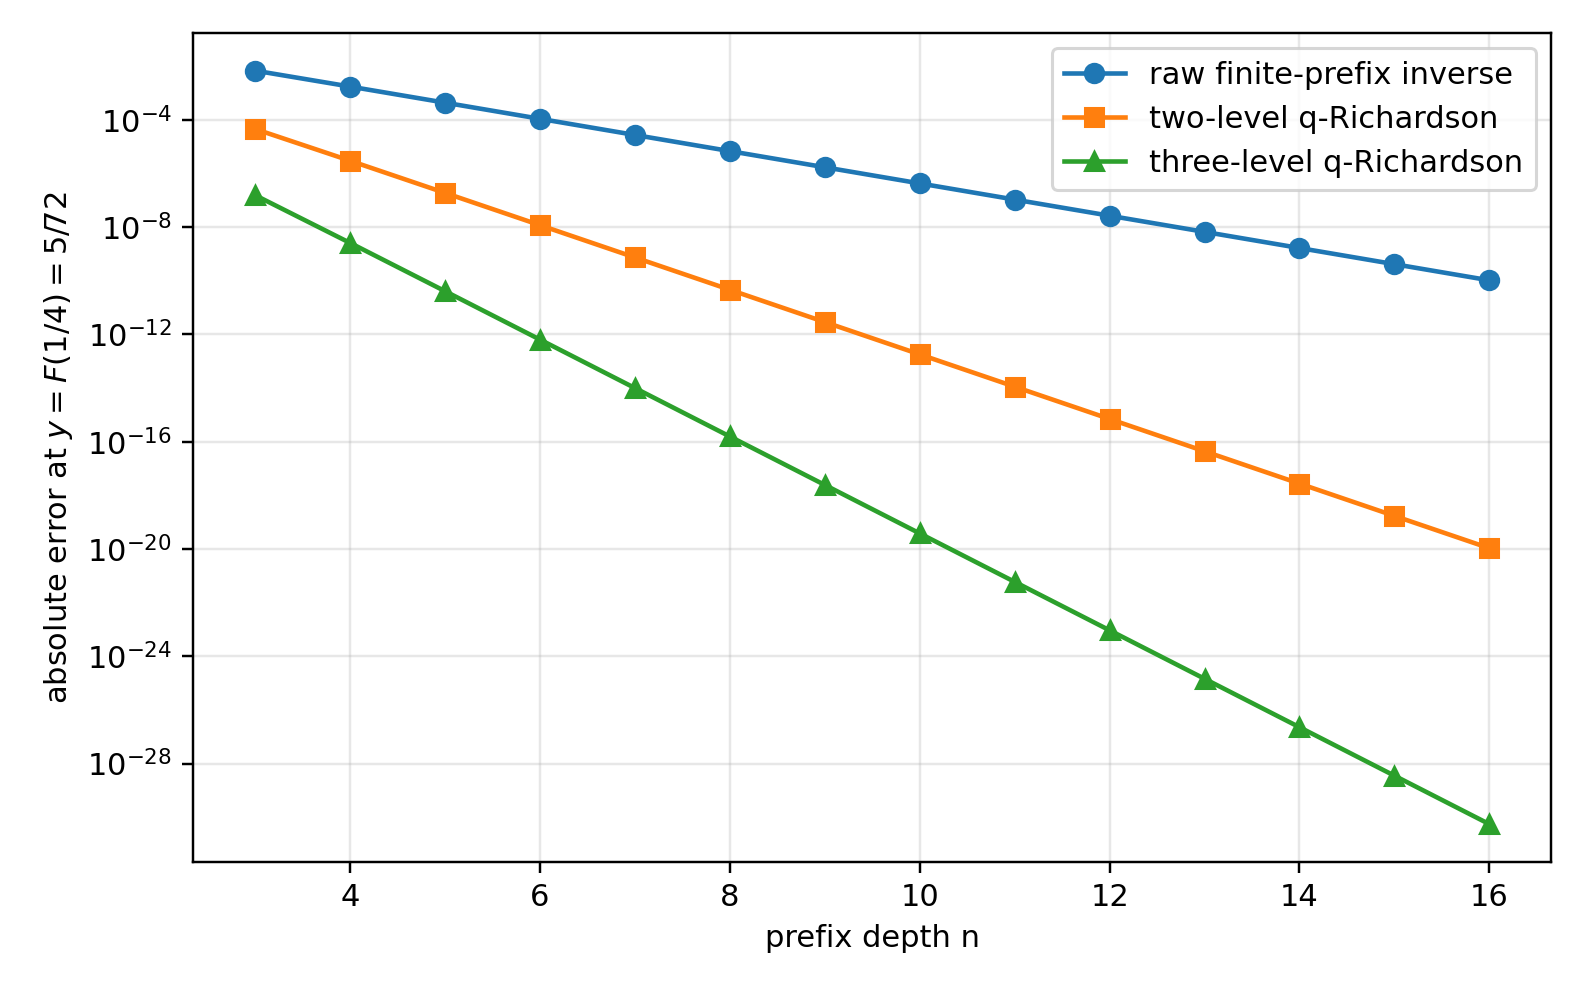
\includegraphics[width=0.92\textwidth]{assets/inverse-germs/figures/quarter_quantile_richardson.png}
\caption{Raw and accelerated errors at the exact output $F(1/4)=5/72$.  The
straight-line separation on the logarithmic scale reflects the exact geometric orders
$4^{-n}$, $16^{-n}$, and $64^{-n}$.}
\label{is:p1:fig:quarter-richardson}
\end{figure}

\subsection{Exact sign and two-sided bounds for every accelerated quarter error}

The preceding asymptotic constants can be strengthened to a finite-$n$ interpolation
statement.  Put
\begin{equation}
 f(Q):=\Delta_2(Q)=\frac{\sqrt{1+(64/9)Q}-1}{8}.
 \label{is:p1:eq:f-quarter-germ}
\end{equation}
For fixed $n$ and $s$, the quantity
$\mathcal G_{n,s}(5/72)-1/4$ is the value at $Q=0$ of the polynomial of degree
at most $s-1$ interpolating $f$ at the nodes
$4^{-n},4^{-(n+1)},\ldots,4^{-(n+s-1)}$.

\begin{theorem}[Positive accelerated errors and sharp finite-depth bounds]
\label{is:p1:thm:quarter-positive-bounds}
Let
\begin{equation}
 K_s:=\frac{C_{s-1}2^{-s^2+5s-2}}{9^s}.
 \label{is:p1:eq:Ks-quarter}
\end{equation}
For every $s\ge1$ and $n\ge3$,
\begin{equation}
 \boxed{
 0< K_s4^{-sn}\left(1+\frac{64}{9}4^{-n}\right)^{\frac12-s}
 <\mathcal G_{n,s}\!\left(\frac5{72}\right)-\frac14
 <K_s4^{-sn}.}
 \label{is:p1:eq:quarter-two-sided}
\end{equation}
In particular, the ratio of the exact error to its leading term is squeezed to one
inside an explicitly shrinking enclosure.
\end{theorem}

\begin{proof}
Let $p_{n,s-1}$ be the Lagrange interpolant just described.  The interpolation
remainder at zero gives a point $\xi_{n,s}\in(0,4^{-n})$ such that
\begin{equation}
 -p_{n,s-1}(0)
 =\frac{f^{(s)}(\xi_{n,s})}{s!}
   \prod_{j=0}^{s-1}(-4^{-(n+j)}).
 \label{is:p1:eq:Lagrange-remainder-quarter}
\end{equation}
Now
\begin{equation}
 f^{(s)}(Q)=\frac1{8}\left(\frac12\right)^{\!\underline{s}}
 \left(\frac{64}{9}\right)^s
 \left(1+\frac{64}{9}Q\right)^{\frac12-s},
 \label{is:p1:eq:f-quarter-derivative}
\end{equation}
where the falling factorial has sign $(-1)^{s-1}$.  The signs in
\eqref{is:p1:eq:Lagrange-remainder-quarter} therefore imply $p_{n,s-1}(0)>0$.
Using
\begin{equation}
 \frac{\left|\left(\frac12\right)^{\!\underline{s}}\right|}{8s!}
 \left(\frac{64}{9}\right)^s4^{-\binom s2}=K_s
 \label{is:p1:eq:Ks-identity}
\end{equation}
produces the middle expression in \eqref{is:p1:eq:quarter-two-sided} with
$\xi_{n,s}$ in place of either endpoint.  Since the exponent $1/2-s$ is
negative, evaluation at $0$ and $4^{-n}$ gives the two strict bounds.
\end{proof}

\begin{remark}
The positivity in \cref{is:p1:thm:quarter-positive-bounds} is not visible term-by-term in
\eqref{is:p1:eq:Catalan-qbinom-full}, whose tail alternates.  It is a consequence of the
complete monotonicity pattern of the derivatives of the square-root germ and the sign
of the Lagrange remainder.  This is one concrete place where exact interpolation gives
more information than formal Richardson cancellation.
\end{remark}

\begin{proposition}[Large-order Catalan coefficients]
\label{is:p1:prop:Catalan-large-order}
The Taylor coefficients of the quarter germ satisfy
\begin{equation}
 \boxed{
 \delta_{2,m}\sim
 (-1)^{m-1}\frac1{16\sqrt\pi}\left(\frac{64}{9}\right)^m m^{-3/2}.}
 \label{is:p1:eq:Catalan-large-order}
\end{equation}
Thus the branch point $Q=-9/64$ controls both the convergence radius and the
$m^{-3/2}$ algebraic prefactor.
\end{proposition}

\begin{proof}
Insert the classical Catalan asymptotic
$C_{m-1}\sim4^{m-1}/(\sqrt\pi\,m^{3/2})$ into
\eqref{is:p1:eq:Catalan-germ}.
\end{proof}

\subsection{A universal first coefficient at every inverse-dyadic anchor}

The leading displacement of the algebraic germ admits a particularly compact expression in
the dyadic moment numbers $d_r$ from \eqref{is:p1:eq:d-def}.

\begin{proposition}[First algebraic-germ coefficient]
\label{is:p1:prop:first-dyadic-germ-coefficient}
For every $r\ge2$,
\begin{equation}
 \boxed{
 \delta_{r,1}
 =\frac1{18}\frac{F''(2^{-r})}{F'(2^{-r})}
 =\frac{2^{r-1}(r-1)d_{r-2}}{9d_{r-1}}>0.}
 \label{is:p1:eq:first-dyadic-germ-coefficient}
\end{equation}
For $r=1$, $\Delta_1\equiv0$ and $\Gn(1/2)=1/2$ exactly.
\end{proposition}

\begin{proof}
The first equality is \eqref{is:p1:eq:c1} evaluated at $x_r$.  Formula
\eqref{is:p1:eq:dyadic-jet} gives
\[
 \frac{F''(x_r)}{F'(x_r)}
 =4\frac{F(2^{2-r})}{F(2^{1-r})}.
\]
Substitute \eqref{is:p1:eq:d-def} at indices $r-2$ and $r-1$ and simplify the powers
of two.  Positivity follows from $d_j>0$.  The case $r=1$ follows from symmetry
of every prefix density.
\end{proof}

The values $4/9$, $8/5$, and $40/9$ in
\eqref{is:p1:eq:Catalan-first}, \eqref{is:p1:eq:Delta3}, and \eqref{is:p1:eq:Delta4} are therefore
not isolated coincidences; they are the first members of a single exact rational
sequence controlled by adjacent dyadic moments.

% Source fragment: Inverse and sampling frontiers; prefix is.
\subsection{The two random series}

Recall the common variables from \cref{is:p1:eq:Y-prefix}: $(V_j)_{j\ge1}$
are independent and uniform on $[0,1]$, while $U_j=2V_j-1$ is uniform on
$[-1,1]$.  Thus
\begin{equation}
 X=\sum_{j\ge1}2^{-j}V_j,
 \qquad
 Y=\sum_{j\ge1}2^{-j}U_j=2X-1.
 \label{is:p2:eq:XY-series}
\end{equation}
Then $F$ is the distribution function of $X$ and $\RvachevUp$ is the density of $Y$.  Their moment
generating functions are entire:
\begin{align}
 L(t)&=\Expectation\EulerE^{tX}
 =\prod_{j\ge1}\frac{\EulerE^{t/2^j}-1}{t/2^j},
 \label{is:p2:eq:L-def}\\
 M(t)&=\Expectation\EulerE^{tY}
 =\prod_{j\ge1}\frac{\sinh(t/2^j)}{t/2^j}
 =\EulerE^{-t}L(2t).
 \label{is:p2:eq:M-def}
\end{align}
Self-similarity gives
\begin{equation}
 L(2t)=\frac{\EulerE^t-1}{t}L(t),
 \qquad
 M(2t)=\frac{\sinh t}{t}M(t).
 \label{is:p2:eq:mgf-refinement}
\end{equation}
On the imaginary axis,
\begin{equation}
 M(2\pi\ImaginaryUnit z)=\prod_{k\ge0}\SincPi(z/2^k)=:\PhiCyc(z),
 \qquad \SincPi u=\frac{\sin(\pi u)}{\pi u}.
 \label{is:p2:eq:M-Phi}
\end{equation}
Thus the moment problem and the infinite sinc product are two restrictions of the same entire
function.

\subsection{Moments and cumulants}

Write $\kappa_n(X)$ and $\kappa_n(Y)$ for cumulants.  The Bernoulli expansion of
$\log((\EulerE^t-1)/t)$ gives
\begin{align}
 \kappa_1(X)&=\frac12,
 &\kappa_{2r}(X)&=\frac{B_{2r}}{2r(4^r-1)},
 &\kappa_{2r+1}(X)&=0\quad(r\ge1),
 \label{is:p2:eq:X-cumulants}\\
 \kappa_1(Y)&=0,
 &\kappa_{2r}(Y)&=\frac{2^{2r-1}B_{2r}}{r(4^r-1)},
 &\kappa_{2r+1}(Y)&=0.
 \label{is:p2:eq:Y-cumulants}
\end{align}
The first centered moments are
\begin{equation}
 m_0=1,
 \quad m_2=\frac19,
 \quad m_4=\frac{19}{675},
 \quad m_6=\frac{583}{59535},
 \quad m_8=\frac{132809}{32531625}.
 \label{is:p2:eq:Y-moments}
\end{equation}
These established rational sequences will become coefficients in the exact finite-prefix expansion.

% Source fragment: Inverse and sampling frontiers; prefix is.
\section{Algebraic Taylor shadows of the inverse Fabius function}
\label{is:p2:sec:inverse-germs}

\subsection{The finite dyadic jet polynomial}

Fix a reduced dyadic point
\begin{equation}
 x_0=\frac{a}{2^N}\in(0,1),
 \qquad a\ \text{odd},
 \qquad y_0=F(x_0).
 \label{is:p2:eq:x0-y0}
\end{equation}
The derivative atlas \eqref{ii:eq:derivative-atlas} gives
\begin{equation}
 f_k:=F^{(k)}(x_0)
 =2^{\binom{k+1}{2}}\ThetaF(2^kx_0),
 \qquad
 Q_{x_0}(h):=\sum_{k=1}^{N}\frac{f_k}{k!}h^k.
 \label{is:p2:eq:Q-dyadic}
\end{equation}
For $k>N$, the argument $2^kx_0$ is an even integer, so the block formula
\eqref{ii:eq:theta-block} gives $F^{(k)}(x_0)=0$.  Hence $y_0+Q_{x_0}$
is the complete Taylor series of $F$ at $x_0$, not merely a finite-order
truncation.  The exact dyadic evaluator in \cref{is:p3:sec:qbinomial} shows
that every $f_k$ is rational.  Moreover $f_1=F'(x_0)>0$.

Define the smooth remainder
\begin{equation}
 \rho_{x_0}(h):=F(x_0+h)-y_0-Q_{x_0}(h).
 \label{is:p2:eq:rho-flat}
\end{equation}
Every derivative of $\rho_{x_0}$ at zero vanishes.  Nevertheless
$\rho_{x_0}$ is not identically zero on any neighborhood: otherwise $F$
would agree locally with a polynomial, contrary to \cref{ne:thm:nowhere}.

\begin{theorem}[Dyadic algebraic inverse germ; \statusnew]
\label{is:p2:thm:algebraic-inverse-germ}
There is a unique real-analytic germ $S_{x_0}$ at zero satisfying
\begin{equation}
 Q_{x_0}(S_{x_0}(z))=z,
 \qquad S_{x_0}(0)=0.
 \label{is:p2:eq:S-inverse}
\end{equation}
It is algebraic over $\RationalNumbers(z)$.  On a neighborhood of zero,
\begin{equation}
 \boxed{
 \FabiusQuantile(y_0+z)
 =x_0+S_{x_0}(z)+R_{x_0}(z),}
 \label{is:p2:eq:G-shadow}
\end{equation}
where $R_{x_0}$ is smooth, flat at zero, and nonzero on every neighborhood
of zero.  Consequently the complete Taylor series of $\FabiusQuantile$ at
$y_0$ has positive radius and an algebraic sum, but that sum does not
represent $\FabiusQuantile$ on any neighborhood.
\end{theorem}

\begin{proof}
Because $Q_{x_0}'(0)=f_1>0$, the real-analytic inverse-function theorem
gives a unique analytic inverse germ $S_{x_0}$.  It satisfies the polynomial
equation $Q_{x_0}(w)-z=0$ over $\RationalNumbers(z)$, so it is algebraic.

Put
\[
 H(z):=\FabiusQuantile(y_0+z)-x_0.
\]
Then $H(0)=0$, $H'(0)=1/f_1>0$, and
\begin{equation}
 z=Q_{x_0}(H(z))+\rho_{x_0}(H(z)).
 \label{is:p2:eq:H-flat-reversion}
\end{equation}
Fa\`a di Bruno's formula shows directly that $\rho_{x_0}\comp H$ is flat:
every term in every derivative at zero contains a derivative of
$\rho_{x_0}$ at $H(0)=0$.  Taking formal Taylor series in
\eqref{is:p2:eq:H-flat-reversion} therefore gives
$Q_{x_0}(\mathsf T_H(z))=z$.  A formal series with zero constant term and
nonzero linear coefficient has a unique compositional inverse; hence
$\mathsf T_H=\mathsf T_{S_{x_0}}$.  Thus
$R_{x_0}:=H-S_{x_0}$ is smooth and flat.

If $R_{x_0}$ vanished throughout some neighborhood, then
$\FabiusQuantile$ would agree there with the analytic germ
$x_0+S_{x_0}$.  Its derivative at $y_0$ is positive, so the analytic
inverse-function theorem would make $F$ analytic at $x_0$, again
contradicting \cref{ne:thm:nowhere}.  Therefore the flat remainder is
nonzero in every neighborhood.  Finally, its vanishing Taylor series shows
that the Taylor series of $\FabiusQuantile$ is precisely the convergent
algebraic series of $S_{x_0}$.
\end{proof}

\begin{resultbox}[Analytic shadow versus the actual inverse]
At each dyadic output $F(a/2^N)$, every derivative of the inverse is encoded
by a finite rational polynomial, yet the actual inverse differs from that
algebraic germ by a nontrivial flat function.  Positive Taylor radius and
local analyticity are therefore sharply different properties here.
\end{resultbox}

\subsection{Lagrange--B\"urmann and Bell formulas}

Factor
\begin{equation}
 Q_{x_0}(u)=u\varphi_{x_0}(u),
 \qquad
 \varphi_{x_0}(0)=f_1>0.
 \label{is:p2:eq:Q-phi}
\end{equation}
The coefficients of the algebraic inverse are completely explicit.

\begin{theorem}[All inverse derivatives at dyadic outputs; \statusnew]
\label{is:p2:thm:inverse-derivatives}
For every $m\ge1$,
\begin{equation}
 \boxed{
 \FabiusQuantile^{(m)}(y_0)
 =(m-1)!\,[u^{m-1}]\,\varphi_{x_0}(u)^{-m}.
 }
 \label{is:p2:eq:Lagrange-inverse-derivative}
\end{equation}
Equivalently, if $g_m=\FabiusQuantile^{(m)}(y_0)$ and $B_{m,k}$ denotes the partial exponential Bell
polynomial, then
\begin{align}
 g_1&=\frac1{f_1},
 \label{is:p2:eq:g1}\\
 g_m&=-\frac1{f_1}
 \sum_{k=2}^{\min(m,N)}f_k
 B_{m,k}(g_1,g_2,\ldots,g_{m-k+1})
 \qquad(m\ge2).
 \label{is:p2:eq:Bell-inverse-recurrence}
\end{align}
In particular, every $\FabiusQuantile^{(m)}(y_0)$ is rational.
\end{theorem}

\begin{proof}
The Lagrange--B\"urmann formula for the inverse of $z=u\varphi_{x_0}(u)$ gives
\[
 [z^m]S_{x_0}(z)=\frac1m[u^{m-1}]\varphi_{x_0}(u)^{-m}.
\]
Multiplication by $m!$ proves \eqref{is:p2:eq:Lagrange-inverse-derivative}.  For the Bell recurrence,
differentiate $F(\FabiusQuantile(y))=y$ $m$ times at $y=y_0$.  Fa\`a di Bruno gives
\[
 \sum_{k=1}^{m} f_k B_{m,k}(g_1,\ldots,g_{m-k+1})=0\qquad(m\ge2).
\]
Since $B_{m,1}=g_m$, solving for the newest derivative gives
\eqref{is:p2:eq:Bell-inverse-recurrence}.  All inputs are rational.
\end{proof}

\begin{remark}
The formulas use two different Bell-polynomial roles in the same theory.  Partial Bell polynomials
invert composition in \eqref{is:p2:eq:Bell-inverse-recurrence}; complete Bell polynomials will invert a
moment generating function in \cref{is:p2:sec:appell}.  The two appearances are not cosmetic variants:
one organizes set partitions by the number of blocks, while the other sums over all block counts.
\end{remark}

\subsection{The midpoint and quarter-point shadows}

At $x_0=y_0=1/2$, reflection gives $F'(1/2)=2$ and makes every higher
derivative vanish.  Thus
\begin{equation}
 Q_{1/2}(h)=2h,
 \qquad
 S_{1/2}(z)=\frac z2,
 \qquad
 \FabiusQuantile(1/2+z)=\frac12+\frac z2+R_{1/2}(z).
 \label{is:p2:eq:midpoint-shadow}
\end{equation}
The reflection law for $\FabiusQuantile$ makes $R_{1/2}$ odd;
\cref{is:p2:thm:algebraic-inverse-germ} makes it flat and nonzero in every
neighborhood.  Hence every derivative beyond the first vanishes even though
the inverse is not affine on any interval.

The first nonlinear shadow has a classical coefficient sequence.

\begin{theorem}[Catalan inverse jet at $F(1/4)$; \statusnew]
\label{is:p2:thm:Catalan-quarter}
One has
\begin{equation}
 F(1/4)=\frac5{72},
 \qquad F'(1/4)=1,
 \qquad F''(1/4)=8,
 \qquad F^{(m)}(1/4)=0\quad(m\ge3).
 \label{is:p2:eq:quarter-jet}
\end{equation}
Consequently
\begin{equation}
 Q_{1/4}(h)=h+4h^2,
 \qquad
 S_{1/4}(z)=\frac{\sqrt{1+16z}-1}{8},
 \label{is:p2:eq:quarter-shadow}
\end{equation}
and, for every $m\ge1$,
\begin{equation}
 \boxed{
 \FabiusQuantile^{(m)}(5/72)
 =m!(-1)^{m-1}4^{m-1}C_{m-1},
 \qquad C_r=\frac1{r+1}\binom{2r}{r}.}
 \label{is:p2:eq:Catalan-derivatives}
\end{equation}
In particular,
\begin{equation}
 \AbsoluteValue{\FabiusQuantile^{(m)}(5/72)}
 \sim\frac{m!\,16^{m-1}}{\sqrt\pi\,(m-1)^{3/2}}.
 \label{is:p2:eq:Catalan-asymptotic}
\end{equation}
\end{theorem}

\begin{proof}
The exact dyadic formula of \cref{is:p3:sec:qbinomial} gives
$F(1/4)=5/72$.  The derivative atlas and the values
$\ThetaF(1/2)=F(1/2)=1/2$ and $\ThetaF(1)=\RvachevUp(0)=1$ give the first
two derivatives in \eqref{is:p2:eq:quarter-jet}.  For $m\ge3$, the argument
$2^m/4$ is an even integer, so \eqref{ii:eq:theta-block} gives zero.
Solving $z=h+4h^2$ for the branch with $h(0)=0$ proves
\eqref{is:p2:eq:quarter-shadow}.  The Catalan generating function, after
the substitution $w=-4z$, is
\[
 \frac{\sqrt{1+16z}-1}{8}
 =\sum_{m\ge1}(-1)^{m-1}4^{m-1}C_{m-1}z^m.
\]
Because the flat remainder has zero derivatives, multiplying the coefficient
of $z^m$ by $m!$ proves \eqref{is:p2:eq:Catalan-derivatives}.  Finally use
$C_r\sim4^r/(\sqrt\pi\,r^{3/2})$.
\end{proof}

For reference, the first values are
\[
 \FabiusQuantile'(5/72)=1,
 \quad \FabiusQuantile''(5/72)=-8,
 \quad \FabiusQuantile^{(3)}(5/72)=192,
 \quad \FabiusQuantile^{(4)}(5/72)=-7680.
\]
These rapidly growing derivatives belong to the algebraic square-root
shadow; they do not assert local analyticity of the actual inverse.

\subsection{The eighth-point cubic and the singularity atlas}

At $x_0=1/8$, exact dyadic evaluation and the derivative atlas give
\begin{equation}
 F(1/8)=\frac1{288},
 \qquad F'(1/8)=\frac5{36},
 \qquad F''(1/8)=4,
 \qquad F^{(3)}(1/8)=64.
 \label{is:p2:eq:eighth-jet}
\end{equation}
Thus the inverse Taylor series at $1/288$ is the origin branch of
\begin{equation}
 z=\frac5{36}h+2h^2+\frac{32}{3}h^3,
 \label{is:p2:eq:eighth-cubic}
\end{equation}
and \cref{is:p2:thm:inverse-derivatives} specializes to
\begin{equation}
 \FabiusQuantile^{(m)}(1/288)
 =(m-1)![u^{m-1}]
 \left(\frac5{36}+2u+\frac{32}{3}u^2\right)^{-m}.
 \label{is:p2:eq:eighth-coeff}
\end{equation}

The finite polynomial $Q_{x_0}$ also turns large-order derivative analysis
into finite algebraic geometry.  Singularities of its inverse branch occur
at critical values $Q_{x_0}(u_c)$ with $Q_{x_0}'(u_c)=0$ (or at infinity).
A nearest simple critical value produces the universal square-root
$m^{-3/2}$ coefficient factor seen above; higher critical multiplicity
produces the corresponding Puiseux exponent.

\begin{problem}[Dyadic inverse singularity atlas]
\label{is:p2:prob:dyadic-singularity-atlas}
For every reduced dyadic $a/2^N$, classify the critical values of
$Q_{a/2^N}$, determine those visible from the origin branch and hence its
exact convergence radius, and describe the Galois and $2$-adic structure of
the associated Puiseux constants.  The cases $N=2$ and $N=3$ are the
quadratic Catalan and cubic examples above.
\end{problem}

% Source fragment: Inverse and sampling frontiers; prefix is.
\section{Kabaya--Iri polynomials and the Rvachev Appell inverse}
\label{is:p2:sec:appell}

\subsection{The external precursor and the normalization used here}

Lee's scaling-polynomial construction associates to a compactly supported probability density
$\phi$ the Appell sequence generated by
$\EulerE^{xt}/\FourierAngular{\phi}(\ImaginaryUnit t)$ and proves its biorthogonality
to the distributional derivatives of $\phi$.  For the up-function, these are the Kabaya--Iri
polynomials.  In the Fabius normalization used in this report, it is convenient to distinguish the
uncentered law $X\in[0,1]$ from the centered law $Y=2X-1\in[-1,1]$.

\begin{definition}[Kabaya--Iri and centered Rvachev--Appell polynomials]
\label{is:p2:def:Appell-polys}
Define $P_n,A_n\in\RationalNumbers[x]$ by
\begin{align}
 \frac{\EulerE^{xt}}{L(t)}
 &=\sum_{n\ge0}P_n(x)\frac{t^n}{n!},
 \label{is:p2:eq:P-generating}\\
 \frac{\EulerE^{xt}}{M(t)}
 &=\sum_{n\ge0}A_n(x)\frac{t^n}{n!}.
 \label{is:p2:eq:A-generating}
\end{align}
\end{definition}

The affine change $M(t)=\EulerE^{-t}L(2t)$ gives
\begin{equation}
 \boxed{
 A_n(x)=2^nP_n\!\left(\frac{x+1}{2}\right),
 \qquad
 P_n(x)=2^{-n}A_n(2x-1).
 }
 \label{is:p2:eq:A-P-affine}
\end{equation}
Thus the sequence $P_n$ is the known Kabaya--Iri sequence, while $A_n$ is its symmetric Rvachev
normalization.  The centering eliminates every odd cumulant and makes the pole analysis in
\cref{is:p2:sec:poles} transparent.

\subsection{Appell, mean-value, and biorthogonality identities}

\begin{proposition}[Classical Appell package; \statuslit]
\label{is:p2:prop:Appell-package}
For $n\ge1$ and, in the biorthogonality identities, every integer $r\ge0$,
\begin{align}
 P_n'(x)&=nP_{n-1}(x),
 &A_n'(x)&=nA_{n-1}(x),
 \label{is:p2:eq:Appell-derivative}\\
 P_n(x+y)&=\sum_{k=0}^n\binom nkP_k(x)y^{n-k},
 &A_n(x+y)&=\sum_{k=0}^n\binom nkA_k(x)y^{n-k}.
 \label{is:p2:eq:Appell-translation}
\end{align}
The polynomial averaging operators are inverted exactly:
\begin{equation}
 \boxed{
 \Expectation\,P_n(x+X)=x^n,
 \qquad
 \Expectation\,A_n(x+Y)=x^n.
 }
 \label{is:p2:eq:mean-value-inversion}
\end{equation}
If $f_X=F'$ is the density of $X$, then in the distributional sense
\begin{equation}
 \left\langle(-1)^r f_X^{(r)},\frac{P_n}{n!}\right\rangle=\delta_{rn}.
 \label{is:p2:eq:P-biorthogonal}
\end{equation}
Equivalently, for the centered density $\RvachevUp$,
\begin{equation}
 \int_{-1}^{1}(-1)^r\RvachevUp^{(r)}(x)\frac{A_n(x)}{n!}\,\Differential x
 =\delta_{rn}.
 \label{is:p2:eq:A-biorthogonal}
\end{equation}
\end{proposition}

\begin{proof}
Differentiate the generating functions with respect to $x$ to obtain
\eqref{is:p2:eq:Appell-derivative}; multiply by $\EulerE^{yt}$ to obtain
\eqref{is:p2:eq:Appell-translation}.  For the mean-value identities,
\[
 \Expectation\sum_{n\ge0}P_n(x+X)\frac{t^n}{n!}
 =\Expectation\frac{\EulerE^{(x+X)t}}{L(t)}=\EulerE^{xt},
\]
and similarly for $A_n$.  Here is the distributional calculation, including
the case in which the order of differentiation exceeds the polynomial degree.
Regard $f_X$ as a compactly supported smooth function on $\RealNumbers$.  By
the definition of a distributional derivative and repeated integration by
parts,
\begin{equation}
 \left\langle(-1)^r f_X^{(r)},\frac{P_n}{n!}\right\rangle
 =\left\langle f_X,
   \left(\frac{P_n}{n!}\right)^{(r)}\right\rangle.
 \label{is:p2:eq:P-biorthogonal-calculation}
\end{equation}
There are no boundary terms in this formulation.  Iterating the Appell rule
shows that the polynomial on the right is
\[
 \left(\frac{P_n}{n!}\right)^{(r)}
 =\begin{cases}
   P_{n-r}/(n-r)!,&0\le r\le n,\\
   0,&r>n.
  \end{cases}
\]
For $r\le n$, the right side of
\eqref{is:p2:eq:P-biorthogonal-calculation} is therefore
\[
 \frac{\Expectation P_{n-r}(X)}{(n-r)!}
 =\delta_{rn},
\]
where the second equality is \eqref{is:p2:eq:mean-value-inversion} at $x=0$
(the expectation is $1$ for $n-r=0$ and $0$ for $n-r>0$); for $r>n$ the
pairing is zero because the test polynomial has vanished.  This proves
\eqref{is:p2:eq:P-biorthogonal} for every $r\ge0$.

For completeness, the centered identity is exactly the affine transport of
this calculation.  Since $Y=2X-1$,
\[
 \RvachevUp(y)=\frac12 f_X\!\left(\frac{y+1}{2}\right),
 \qquad
 \RvachevUp^{(r)}(y)=2^{-r-1}f_X^{(r)}\!\left(\frac{y+1}{2}\right),
\]
while \eqref{is:p2:eq:A-P-affine} gives
$A_n(y)=2^nP_n((y+1)/2)$.  Thus the substitution $y=2u-1$ gives
\begin{align*}
 \int_{-1}^{1}(-1)^r\RvachevUp^{(r)}(y)
       \frac{A_n(y)}{n!}\,\Differential y
 &=2^{n-r}
   \left\langle(-1)^r f_X^{(r)},\frac{P_n}{n!}\right\rangle\\
 &=2^{n-r}\delta_{rn}=\delta_{rn},
\end{align*}
which is \eqref{is:p2:eq:A-biorthogonal}.
\end{proof}

\begin{remark}
Equation \eqref{is:p2:eq:mean-value-inversion} is an exact polynomial deconvolution formula.  The operator
$\mathcal T_Y:p\mapsto\Expectation p(\,\cdot+Y)$ is triangular on $\RationalNumbers[x]$ with ones on its diagonal;
$A_n=\mathcal T_Y^{-1}x^n$.  This is the linear inverse problem paired with
quantile inversion in the common platform of \cref{sec:common-platform}.
\end{remark}

\subsection{Bell reconstruction from Bernoulli cumulants}

Set
\begin{equation}
 \alpha_n=A_n(0),
 \qquad
 \frac1{M(t)}=\sum_{n\ge0}\alpha_n\frac{t^n}{n!}.
 \label{is:p2:eq:alpha-def}
\end{equation}
Symmetry gives $\alpha_{2r+1}=0$.  If $\ExponentialCompleteBellPolynomial{n}$ denotes the complete exponential Bell polynomial,
then \eqref{is:p2:eq:Y-cumulants} yields
\begin{equation}
 \boxed{
 \alpha_n=\ExponentialCompleteBellPolynomial{n}\bigl(-\kappa_1(Y),-\kappa_2(Y),\ldots,-\kappa_n(Y)\bigr).
 }
 \label{is:p2:eq:alpha-Bell}
\end{equation}
Equivalently,
\begin{equation}
 \alpha_0=1,
 \qquad
 \alpha_n=-\sum_{j=1}^n\binom{n-1}{j-1}\kappa_j(Y)\alpha_{n-j}.
 \label{is:p2:eq:alpha-recurrence}
\end{equation}
The first constants are
\begin{equation}
 \alpha_0=1,
 \quad \alpha_2=-\frac19,
 \quad \alpha_4=\frac{31}{675},
 \quad \alpha_6=-\frac{2347}{59535},
 \quad \alpha_8=\frac{1904369}{32531625}.
 \label{is:p2:eq:alpha-first}
\end{equation}
The Appell translation law then gives
\begin{equation}
 A_n(x)=\sum_{k=0}^n\binom nk\alpha_{n-k}x^k.
 \label{is:p2:eq:A-from-alpha}
\end{equation}
For reference,
\begin{equation}
\begin{aligned}
 A_0(x)&=1,\\
 A_1(x)&=x,\\
 A_2(x)&=x^2-\frac19,\\
 A_3(x)&=x^3-\frac13x,\\
 A_4(x)&=x^4-\frac23x^2+\frac{31}{675},\\
 A_5(x)&=x^5-\frac{10}{9}x^3+\frac{31}{135}x,\\
 A_6(x)&=x^6-\frac53x^4+\frac{31}{45}x^2-\frac{2347}{59535}.
\end{aligned}
\label{is:p2:eq:A-first-polys}
\end{equation}
Using \eqref{is:p2:eq:A-P-affine}, the first uncentered polynomials are
\begin{equation}
\begin{aligned}
 P_0(x)&=1,\\
 P_1(x)&=x-\frac12,\\
 P_2(x)&=x^2-x+\frac29,\\
 P_3(x)&=x^3-\frac32x^2+\frac23x-\frac1{12},\\
 P_4(x)&=x^4-2x^3+\frac43x^2-\frac13x+\frac{16}{675},\\
 P_5(x)&=x^5-\frac52x^4+\frac{20}{9}x^3-\frac56x^2+\frac{16}{135}x-\frac1{270}.
\end{aligned}
\label{is:p2:eq:P-first-polys}
\end{equation}
These agree with Lee's displayed Kabaya--Iri list through degree five.

\subsection{Bernoulli refinement recurrences}

The self-similarity identities \eqref{is:p2:eq:mgf-refinement} become polynomial recurrences when the
reciprocal generating functions are compared.

\begin{proposition}[Bernoulli refinement of the Appell sequences]
\label{is:p2:prop:Bernoulli-refinement}
Let $B_k$ be defined by $t/(\EulerE^t-1)=\sum B_kt^k/k!$, and let
$c_{2r}=2(1-2^{2r-1})B_{2r}$ be the exponential coefficients of
$t/\sinh t$.  Then
\begin{align}
 2^nP_n(x)
 &=\sum_{k=0}^n\binom nkB_kP_{n-k}(2x),
 \label{is:p2:eq:P-Bernoulli-refinement}\\
 2^nA_n(x)
 &=\sum_{r=0}^{\Floor{n/2}}
   \binom n{2r}c_{2r}A_{n-2r}(2x).
 \label{is:p2:eq:A-Bernoulli-refinement}
\end{align}
\end{proposition}

\begin{proof}
Substitute \eqref{is:p2:eq:mgf-refinement} into the defining generating functions:
\begin{align*}
 \frac{\EulerE^{2xt}}{L(2t)}
 &=\frac{t}{\EulerE^t-1}\frac{\EulerE^{2xt}}{L(t)},\\
 \frac{\EulerE^{2xt}}{M(2t)}
 &=\frac{t}{\sinh t}\frac{\EulerE^{2xt}}{M(t)}.
\end{align*}
Coefficient comparison gives the two formulas.
\end{proof}

\begin{remark}
The repository's Bernoulli recurrences usually govern moments, reciprocal sine products, or saddle
coefficients.  Here the same Bernoulli numbers govern a polynomial eigenbasis for the adjoint
Rvachev averaging operator.  The recurrence is a direct algebraic shadow of dyadic refinement.
\end{remark}

\subsection{A dyadic logistic dual}

The complete Bell signs in \eqref{is:p2:eq:alpha-first} admit a probabilistic explanation that appears not
to have been recorded for the Rvachev law.

Let $\Lambda$ be a standard logistic random variable with density
\begin{equation}
 \ell(x)=\frac{\EulerE^{-x}}{(1+\EulerE^{-x})^2}.
 \label{is:p2:eq:logistic-density}
\end{equation}
The beta integral gives
\begin{equation}
 \Expectation\EulerE^{\ImaginaryUnit t\Lambda}
 =\Gamma(1+\ImaginaryUnit t)\Gamma(1-\ImaginaryUnit t)
 =\frac{\pi t}{\sinh(\pi t)}.
 \label{is:p2:eq:logistic-cf}
\end{equation}
Let $(\Lambda_j)_{j\ge1}$ be independent copies and define
\begin{equation}
 Z=\sum_{j\ge1}\frac{\Lambda_j}{\pi2^j}.
 \label{is:p2:eq:Z-logistic}
\end{equation}
The series converges in $L^2$ and almost surely.

\begin{theorem}[Logistic dual of the Rvachev law; \statusnew]
\label{is:p2:thm:logistic-dual}
For real $t$,
\begin{equation}
 \boxed{
 \Expectation\EulerE^{\ImaginaryUnit tZ}
 =\prod_{j\ge1}\frac{t/2^j}{\sinh(t/2^j)}
 =\frac1{M(t)}.
 }
 \label{is:p2:eq:Z-cf}
\end{equation}
Consequently, as polynomial identities,
\begin{align}
 A_n(x)&=\Expectation\,(x+\ImaginaryUnit Z)^n,
 \label{is:p2:eq:A-logistic-moment}\\
 P_n(x)&=\Expectation\left(x-\frac12+\frac{\ImaginaryUnit Z}{2}\right)^n.
 \label{is:p2:eq:P-logistic-moment}
\end{align}
In particular,
\begin{equation}
 \boxed{
 \alpha_{2m}=(-1)^m\Expectation Z^{2m},
 \qquad (-1)^m\alpha_{2m}>0.
 }
 \label{is:p2:eq:alpha-sign}
\end{equation}
\end{theorem}

\begin{proof}
We first record the integrability needed to turn the formal coefficient
comparison into an analytic one.  The logistic density satisfies
$\ell(x)\le\EulerE^{-\AbsoluteValue{x}}$, so
$\Expectation\EulerE^{s\AbsoluteValue{\Lambda}}<\infty$ for $0\le s<1$.
Fix $0<a<2\pi$ and put $s_j=a/(\pi2^j)$.  Since
\[
 \log\Expectation\EulerE^{s\AbsoluteValue{\Lambda}}=\BigO(s)
 \qquad(s\downarrow0),
\]
independence and monotone convergence give
\begin{equation}
 \Expectation\exp\!\left(
   a\sum_{j\ge1}\frac{\AbsoluteValue{\Lambda_j}}{\pi2^j}
  \right)
 =\prod_{j\ge1}\Expectation\EulerE^{s_j\AbsoluteValue{\Lambda}}
 <\infty.
 \label{is:p2:eq:Z-exponential-moment}
\end{equation}
In particular, the defining series for $Z$ converges absolutely almost surely
and $\Expectation\EulerE^{a\AbsoluteValue Z}<\infty$ for every
$0<a<2\pi$.

Let $Z_N=\sum_{j=1}^N\Lambda_j/(\pi2^j)$.  Independence and
\eqref{is:p2:eq:logistic-cf} give, for real $t$,
\[
 \Expectation\EulerE^{\ImaginaryUnit tZ_N}
 =\prod_{j=1}^{N}\frac{t/2^j}{\sinh(t/2^j)}.
\]
The almost-sure convergence $Z_N\to Z$ and bounded convergence pass the left
side to $\Expectation\EulerE^{\ImaginaryUnit tZ}$.  On the right,
\[
 \log\!\left(\frac{w}{\sinh w}\right)=\BigO(w^2)
 \qquad(w\to0),
\]
so the product converges locally uniformly for complex $t$ in
$\AbsoluteValue t<2\pi$; its factors are nonzero there, and its product is
the reciprocal of the locally uniformly convergent product defining $M(t)$.
The exponential-moment bound makes
$t\mapsto\Expectation\EulerE^{\ImaginaryUnit tZ}$ holomorphic on every strip
$\AbsoluteValue{\operatorname{Im}t}<a<2\pi$.  Thus the identity theorem
extends the equality from real $t$ throughout the disk
$\AbsoluteValue t<2\pi$, and in particular proves \eqref{is:p2:eq:Z-cf}.

It remains to justify coefficient comparison.  The exponential-moment bound
\eqref{is:p2:eq:Z-exponential-moment} makes
\[
 t\longmapsto \Expectation\EulerE^{t(x+\ImaginaryUnit Z)}
\]
analytic near zero.  Indeed, on any smaller closed disk and for every $n$,
the $n$th derivative of the integrand is dominated by
\[
 (\AbsoluteValue x+\AbsoluteValue Z)^n
 \EulerE^{r(\AbsoluteValue x+\AbsoluteValue Z)},
\]
which is integrable after choosing $r<a<2\pi$.  Differentiation under the
expectation is therefore valid to every order.  Consequently
\[
 \frac{\EulerE^{xt}}{M(t)}
 =\EulerE^{xt}\Expectation\EulerE^{\ImaginaryUnit tZ}
 =\Expectation\EulerE^{t(x+\ImaginaryUnit Z)}
 =\sum_{n\ge0}\Expectation(x+\ImaginaryUnit Z)^n\frac{t^n}{n!}
\]
near zero, and comparison with \eqref{is:p2:eq:A-generating} proves
\eqref{is:p2:eq:A-logistic-moment} for every real $x$, hence as a polynomial
identity.  Substituting $2x-1$ and using
\eqref{is:p2:eq:A-P-affine} gives \eqref{is:p2:eq:P-logistic-moment}.
Finally $Z$ is symmetric and nondegenerate; indeed, independence and
$\Variance(\Lambda)=\pi^2/3$ give
$\Variance(Z)=\sum_{j\ge1}(3\cdot4^j)^{-1}=1/9$.
Therefore setting $x=0$ gives
$\alpha_{2m}=(-1)^m\Expectation Z^{2m}$ and
$\Expectation Z^{2m}>0$ (with the value $1$ when $m=0$), proving
\eqref{is:p2:eq:alpha-sign}.
\end{proof}

\begin{resultbox}[A duality of compact and noncompact laws]
The Rvachev variable $Y$ is compactly supported and has moment generating function $M$.  Its
polynomial deconvolution sequence is represented by imaginary moments of the noncompact variable
$Z$, an infinite dyadic sum of logistic variables, whose characteristic function is $M^{-1}$.
Thus $M(t)^{-1}=\PhiAng(-\ImaginaryUnit t)^{-1}$ is not merely a formal
series: on the real $t$-axis it is the positive-definite characteristic
function of $Z$.  This is the reciprocal \emph{hyperbolic}-sinc product, or
equivalently the analytic continuation of the reciprocal trigonometric-sinc
product to the imaginary Fourier axis.  The function $1/\PhiAng(\xi)$ on the
real Fourier axis has poles and is not a characteristic function.
\end{resultbox}

\subsection{Operator interpretation}

Let $D=\Differential/\Differential x$.  On polynomials,
\begin{equation}
 \mathcal T_Y=\Expectation\EulerE^{YD}=M(D),
 \qquad
 \mathcal T_Y^{-1}=M(D)^{-1}=\Expectation\EulerE^{\ImaginaryUnit ZD}.
 \label{is:p2:eq:operator-deconvolution}
\end{equation}
Therefore
\begin{equation}
 A_n=M(D)^{-1}x^n.
 \label{is:p2:eq:A-operator}
\end{equation}
This identity packages the mean-value theorem, the logistic dual, and the Appell derivative rule in
one line.  It also prepares the finite Barnes and Thue--Morse difference calculus: replacing $M$ by
a finite product replaces the infinite-order differential operator by a finite product of Bernoulli
operators.

\section{Exact distribution laws for all Rvachev derivatives}
\label{rvd:sec:derivative-distribution}

The latest formal development yields a distributional theorem stronger than
any individual derivative norm or moment identity.  It is logically distinct
from Appell biorthogonality: the test function below is applied to the
\emph{value} of a derivative, not multiplied by an Appell polynomial in the
spatial variable.

For $n\ge0$, $0\le k<2^n$, and $-1\le y\le1$, put
\[
 c_{n,k}(y):=-1+\frac{2k+1+y}{2^n},
 \qquad \mathcal D_n:=2^{\binom{n+1}{2}},
\]
and let $\BinaryDigitSum(k)$ be the binary digit sum.

\begin{theorem}[Cell tiling and derivative pushforward laws]
\label{rvd:thm:derivative-distribution}
The $n$th derivative of the Rvachev function $u$ satisfies
\begin{equation}
 u^{(n)}(c_{n,k}(y))=\mathcal D_n(-1)^{\BinaryDigitSum(k)}u(y).
 \label{rvd:eq:cell-tiling}
\end{equation}
Consequently, for every continuous real- or Banach-valued test function $H$,
\begin{equation}
 \int_{-1}^{1}H\!\left(\mathcal D_n^{-1}|u^{(n)}(x)|\right)\Differential x
 =\int_{-1}^{1}H(u(y))\Differential y.
 \label{rvd:eq:absolute-law}
\end{equation}
For $n\ge1$ the signed normalized law is the symmetric half-mixture
\begin{equation}
 \int_{-1}^{1}H\!\left(\mathcal D_n^{-1}u^{(n)}(x)\right)\Differential x
 =\frac12\int_{-1}^{1}\bigl(H(u(y))+H(-u(y))\bigr)\Differential y.
 \label{rvd:eq:signed-law}
\end{equation}
Equivalently, these are equalities of Borel pushforward measures under
Lebesgue measure restricted to $[-1,1]$.  In particular, for $m\in\NaturalNumbers$,
\begin{equation}
 \int_{-1}^{1}(u^{(n)}(x))^m\Differential x
 =2^{-n}(1+(-1)^m)^n\mathcal D_n^m
  \int_{-1}^{1}u(y)^m\Differential y,
 \label{rvd:eq:signed-moments}
\end{equation}
and, for every real $p\ge0$,
\begin{equation}
 \int_{-1}^{1}|u^{(n)}(x)|^p\Differential x
 =\mathcal D_n^p\int_{-1}^{1}u(y)^p\Differential y.
 \label{rvd:eq:absolute-moments}
\end{equation}
\end{theorem}

\begin{proof}
The derivative atlas gives exactly \eqref{rvd:eq:cell-tiling}; the affine map
$c_{n,k}$ carries $[-1,1]$ onto the $k$th of the $2^n$ adjacent level-$n$
cells and has Jacobian $2^{-n}$.  Partitioning $[-1,1]$ into these cells and
substituting $x=c_{n,k}(y)$ therefore gives
\[
 \int_{-1}^{1}H(u^{(n)}(x))\Differential x
 =2^{-n}\sum_{k=0}^{2^n-1}
   \int_{-1}^{1}H\!\left(\mathcal D_n(-1)^{\BinaryDigitSum(k)}u(y)\right)\Differential y.
\]
Taking absolute values erases every sign, and the $2^n$ equal summands cancel
the Jacobian, proving \eqref{rvd:eq:absolute-law}.  For $n\ge1$, toggling the
lowest binary digit pairs the indices with opposite Thue--Morse signs; hence
exactly $2^{n-1}$ signs are positive and $2^{n-1}$ are negative.  This proves
\eqref{rvd:eq:signed-law}.  Continuous test functions determine finite Borel
measures on the compact range, so the integral identities imply the stated
pushforward equalities.  Finally take $H(t)=t^m$ and use the Boolean-cube
identity
\[
 \sum_{k=0}^{2^n-1}\bigl((-1)^m\bigr)^{\BinaryDigitSum(k)}
 =(1+(-1)^m)^n
\]
to obtain \eqref{rvd:eq:signed-moments}; take $H(t)=t^p$ in the nonnegative
absolute law to obtain \eqref{rvd:eq:absolute-moments}.
\end{proof}

The cell identity, Banach-valued test-function formulas, both pushforward
equalities, and all nonnegative real absolute moments are machine checked in
\path{FabiusFunction.RvachevDerivativeDistribution}; the principal
declarations are \path{iteratedDeriv_rvachev_cell},
\path{map_normalized_iteratedDeriv_rvachev_restrict_Icc}, and
\path{map_normalized_abs_iteratedDeriv_rvachev_restrict_Icc}.

\section{Finite dyadic prefixes as Barnes--Bernoulli polynomials}
\label{is:p2:sec:barnes}

\subsection{Finite random sums and finite Appell inverses}

For $N\ge0$, define the convolution prefixes
\begin{equation}
 X_N=\sum_{j=1}^{N}2^{-j}V_j,
 \qquad
 Y_N=\sum_{j=1}^{N}2^{-j}U_j,
 \label{is:p2:eq:finite-XY}
\end{equation}
with the empty-sum convention $X_0=Y_0=0$.  Empty products below are one,
so $L_0=M_0=1$ and $P_n^{[0]}(x)=A_n^{[0]}(x)=x^n$.  This convention makes
depth zero the identity averaging operator and will be used in the exact
interpolation statements.  Their moment generating functions are
\begin{align}
 L_N(t)&=\prod_{j=1}^{N}\frac{\EulerE^{t/2^j}-1}{t/2^j},
 \label{is:p2:eq:LN}\\
 M_N(t)&=\prod_{j=1}^{N}\frac{\sinh(t/2^j)}{t/2^j}.
 \label{is:p2:eq:MN}
\end{align}
Define finite-prefix Appell polynomials by
\begin{align}
 \frac{\EulerE^{xt}}{L_N(t)}
 &=\sum_{n\ge0}P_n^{[N]}(x)\frac{t^n}{n!},
 \label{is:p2:eq:PN-generating}\\
 \frac{\EulerE^{xt}}{M_N(t)}
 &=\sum_{n\ge0}A_n^{[N]}(x)\frac{t^n}{n!}.
 \label{is:p2:eq:AN-generating}
\end{align}
They satisfy the exact finite mean-value identities
\begin{equation}
 \Expectation P_n^{[N]}(x+X_N)=x^n,
 \qquad
 \Expectation A_n^{[N]}(x+Y_N)=x^n.
 \label{is:p2:eq:finite-mean-value}
\end{equation}
Because $X_N$ and $Y_N$ are finite convolutions of boxes, these polynomials are the exact
polynomial duals of the spline approximants developed elsewhere in the repository.

\subsection{Normalized Barnes multiple Bernoulli polynomials}

For nonzero periods $b_1,\ldots,b_N$, define the normalized Barnes multiple Bernoulli polynomials
$\mathfrak B_n^{(N)}$ by
\begin{equation}
 \EulerE^{xt}\prod_{j=1}^{N}\frac{b_jt}{\EulerE^{b_jt}-1}
 =\sum_{n\ge0}
 \mathfrak B_n^{(N)}(x\mid b_1,\ldots,b_N)\frac{t^n}{n!}.
 \label{is:p2:eq:Barnes-def}
\end{equation}
This normalization has leading coefficient one and reduces to the ordinary Bernoulli polynomial
when $N=1$ and $b_1=1$.

\begin{theorem}[Dyadic Barnes identification; \statusnew]
\label{is:p2:thm:Barnes-identification}
For every $N,n\ge0$,
\begin{equation}
 \boxed{
 P_n^{[N]}(x)
 =\mathfrak B_n^{(N)}
 \left(x\mid 2^{-1},2^{-2},\ldots,2^{-N}\right).
 }
 \label{is:p2:eq:P-Barnes}
\end{equation}
Let
\begin{equation}
 s_N=1-2^{-N},
 \qquad
 (a_1,\ldots,a_N)=(1,1/2,\ldots,2^{1-N}).
 \label{is:p2:eq:a-sN}
\end{equation}
Then
\begin{equation}
 \boxed{
 A_n^{[N]}(x)
 =\mathfrak B_n^{(N)}
 \left(x+s_N\mid1,\frac12,\ldots,2^{1-N}\right).
 }
 \label{is:p2:eq:A-Barnes}
\end{equation}
\end{theorem}

\begin{proof}
Equation \eqref{is:p2:eq:P-Barnes} is immediate by comparing
\eqref{is:p2:eq:PN-generating} with \eqref{is:p2:eq:Barnes-def}.  For the centered product, write
\[
 \frac{\sinh(a_jt/2)}{a_jt/2}
 =\EulerE^{-a_jt/2}\frac{\EulerE^{a_jt}-1}{a_jt}.
\]
Since $\frac12\sum_{j=1}^{N}a_j=s_N$, one has
\[
 \frac{\EulerE^{xt}}{M_N(t)}
 =\EulerE^{(x+s_N)t}\prod_{j=1}^{N}\frac{a_jt}{\EulerE^{a_jt}-1},
\]
which is \eqref{is:p2:eq:A-Barnes}.
\end{proof}

\begin{remark}
The period vectors are geometric rather than repeated.  This is a Barnes analogue of the
repository's ubiquitous $q=1/2$ geometry: each new convolution scale appends one period to the
multiple Bernoulli polynomial.  The infinite Kabaya--Iri sequence is therefore a geometric-period
limit of a Barnes tower.
\end{remark}

\subsection{A complete Thue--Morse difference operator}

For a step $h$, write $E_h=\EulerE^{hD}$ for translation: $(E_hp)(x)=p(x+h)$.  The complete binary
signed difference operator is
\begin{equation}
 \Delta_N^{\mathrm{TM}}(b_1,\ldots,b_N)
 :=\prod_{j=1}^{N}(1-E_{b_j}).
 \label{is:p2:eq:TM-operator}
\end{equation}
Expanding the product assigns a sign $(-1)^{|J|}$ to each subset $J$.  With geometric steps, subset
sums are binary integers and the signs are precisely Thue--Morse.

\begin{theorem}[Uncentered Thue--Morse--Barnes collapse; \statusnew]
\label{is:p2:thm:TM-uncentered}
Let $\eps_k=(-1)^{\BinaryDigitSum(k)}$.  For every $N\ge1$ and $n\ge0$,
\begin{equation}
 \boxed{
 \sum_{k=0}^{2^N-1}\eps_k
 P_n^{[N]}\!\left(x+\frac{k}{2^N}\right)
 =(-1)^N2^{-N(N+1)/2}\FallingFactorial{n}{N}\,x^{n-N},
 }
 \label{is:p2:eq:TM-P-collapse}
\end{equation}
where the right side is interpreted as zero when $n<N$.
\end{theorem}

\begin{proof}
Multiply the generating function \eqref{is:p2:eq:PN-generating} by the complete signed exponential sum:
\begin{align*}
 \sum_{k=0}^{2^N-1}\eps_k
 \frac{\EulerE^{(x+k/2^N)t}}{L_N(t)}
 &=\frac{\EulerE^{xt}}{L_N(t)}
   \prod_{j=1}^{N}(1-\EulerE^{t/2^j})\\
 &=(-1)^N\EulerE^{xt}t^N\prod_{j=1}^{N}2^{-j}\\
 &=(-1)^N2^{-N(N+1)/2}t^N\EulerE^{xt}.
\end{align*}
The coefficient of $t^n/n!$ is the stated monomial.
\end{proof}

\begin{corollary}[Prouhet cancellation with a canonical correction]
\label{is:p2:cor:Prouhet-canonical}
For $n<N$, the complete Thue--Morse sum in \eqref{is:p2:eq:TM-P-collapse} vanishes.  For $n=N$, it is the
constant
\begin{equation}
 (-1)^NN!\,2^{-N(N+1)/2}.
 \label{is:p2:eq:TM-first-nonzero}
\end{equation}
For $n>N$, it is exactly the monomial response of an $N$th finite difference.  Thus the finite
Kabaya--Iri polynomial is a canonical polynomial on which the Prouhet cancellation defect is
completely diagonalized.
\end{corollary}

\begin{proof}
Specialize \eqref{is:p2:eq:TM-P-collapse}.  The falling factorial
$\FallingFactorial{n}{N}$ is zero for $n<N$.  At $n=N$ it equals $N!$ and $x^{n-N}=1$,
which gives \eqref{is:p2:eq:TM-first-nonzero}.  When $n>N$, the same formula
is a constant multiple of $x^{n-N}$; this is precisely the response of the
$N$th finite-difference operator to a degree-$n$ Appell polynomial.
\end{proof}

The centered form is sign-cleaner because the support is arranged symmetrically.

\begin{theorem}[Centered Thue--Morse--Rvachev collapse; \statusnew]
\label{is:p2:thm:TM-centered}
With $s_N=1-2^{-N}$, for every $N\ge1$ and $n\ge0$,
\begin{equation}
 \boxed{
 \sum_{k=0}^{2^N-1}\eps_k
 A_n^{[N]}\!\left(x+s_N-\frac{k}{2^{N-1}}\right)
 =2^{-N(N-1)/2}\FallingFactorial{n}{N}\,x^{n-N}.
 }
 \label{is:p2:eq:TM-A-collapse}
\end{equation}
\end{theorem}

\begin{proof}
The binary subset sums of the period vector
$(1,1/2,\ldots,2^{1-N})$ are $k/2^{N-1}$.  Hence
\begin{align*}
 &\sum_{k=0}^{2^N-1}\eps_k
 \frac{\EulerE^{(x+s_N-k/2^{N-1})t}}{M_N(t)}\\
 &\qquad=
 \frac{\EulerE^{(x+s_N)t}}{M_N(t)}
 \prod_{j=1}^{N}(1-\EulerE^{-a_jt}).
\end{align*}
Now
\[
 \prod_{j=1}^{N}(1-\EulerE^{-a_jt})
 =\EulerE^{-2s_Nt}\prod_{j=1}^{N}(\EulerE^{a_jt}-1),
\]
while
\[
 M_N(t)^{-1}=\EulerE^{s_Nt}\prod_{j=1}^{N}\frac{a_jt}{\EulerE^{a_jt}-1}.
\]
All exponentials cancel, leaving
$\EulerE^{xt}t^N\prod_ja_j=2^{-N(N-1)/2}t^N\EulerE^{xt}$.  Coefficient comparison proves the theorem.
\end{proof}

\begin{example}[The first genuinely centered identity]
For $N=2$,
\begin{equation}
 A_4^{[2]}(x)=x^4-\frac58x^2+\frac{53}{1280}.
 \label{is:p2:eq:A4N2}
\end{equation}
The four-point Thue--Morse difference is
\begin{align}
 &A_4^{[2]}(x+3/4)-A_4^{[2]}(x+1/4)
 -A_4^{[2]}(x-1/4)+A_4^{[2]}(x-3/4)
 \notag\\
 &\hspace{5cm}=6x^2.
 \label{is:p2:eq:A4N2-example}
\end{align}
The constants and lower even powers disappear exactly, not asymptotically.
\end{example}

\subsection{A q-binomial form of the difference operator}

The Thue--Morse block polynomial
\begin{equation}
 T_N(z)=\sum_{k=0}^{2^N-1}\eps_kz^k
 =\prod_{r=0}^{N-1}(1-z^{2^r})
 \label{is:p2:eq:TN}
\end{equation}
encodes the same operation as \eqref{is:p2:eq:TM-operator}.  The collapse theorems can therefore be read
in three interchangeable languages:
\begin{equation}
 \text{binary subset signs}
 \longleftrightarrow
 \text{Thue--Morse block polynomial}
 \longleftrightarrow
 \text{product of Barnes difference factors}.
 \label{is:p2:eq:three-languages}
\end{equation}
This is a new bridge between the formula atlas and the finite convolution/Barnes hierarchy.  It also
suggests a higher-rank extension: replace the simple product of differences by the Pascal-weighted
multiplicities of the repository's rank-$r$ Rvachev hierarchy, which should produce multiple
Thue--Morse--Barnes operators with repeated geometric periods.

\section{Exact finite-prefix expansions and \texorpdfstring{$q$}{q}-Richardson recovery}
\label{is:p2:sec:richardson}

\subsection{Tail self-similarity is polynomial in the truncation scale}

Let $X',Y'$ be independent copies of $X,Y$, independent of the first $N$ summands.  Splitting the
random series after level $N$ gives the exact distributional identities
\begin{equation}
 X\overset{d}=X_N+2^{-N}X',
 \qquad
 Y\overset{d}=Y_N+2^{-N}Y'.
 \label{is:p2:eq:tail-self-similarity}
\end{equation}
Hence
\begin{equation}
 L(t)=L_N(t)L(2^{-N}t),
 \qquad
 M(t)=M_N(t)M(2^{-N}t).
 \label{is:p2:eq:finite-infinite-mgf}
\end{equation}
Write $\mu_r=\Expectation X^r$ and $m_{2r}=\Expectation Y^{2r}$.

\begin{theorem}[Exact finite-prefix expansion; \statusnew]
\label{is:p2:thm:finite-prefix-expansion}
For every $N,n\ge0$,
\begin{equation}
 \boxed{
 P_n^{[N]}(x)
 =\sum_{r=0}^{n}\binom nr\mu_r\,2^{-Nr}P_{n-r}(x).
 }
 \label{is:p2:eq:P-prefix-expansion}
\end{equation}
For the centered sequence,
\begin{equation}
 \boxed{
 A_n^{[N]}(x)
 =\sum_{r=0}^{\Floor{n/2}}
 \binom n{2r}m_{2r}\,4^{-Nr}A_{n-2r}(x).
 }
 \label{is:p2:eq:A-prefix-expansion}
\end{equation}
Equivalently, before specializing \(x\), \(P_n^{[N]}\) is exactly a
\(\mathbb Q[x]\)-valued polynomial of degree \(n\) in \(2^{-N}\), while
\(A_n^{[N]}\) is exactly a \(\mathbb Q[x]\)-valued polynomial of degree
\(\Floor{n/2}\) in \(4^{-N}\).  The uncentered degree remains exact after a
fixed-\(x\) specialization, but the centered degree can drop: for odd \(n\),
the leading coefficient contains \(A_1(x)=x\) and vanishes at \(x=0\).
\end{theorem}

\begin{proof}
From \eqref{is:p2:eq:finite-infinite-mgf},
\begin{align*}
 \frac{\EulerE^{xt}}{L_N(t)}
 &=L(2^{-N}t)\frac{\EulerE^{xt}}{L(t)},\\
 \frac{\EulerE^{xt}}{M_N(t)}
 &=M(2^{-N}t)\frac{\EulerE^{xt}}{M(t)}.
\end{align*}
Expand the first extra factor in moments and compare exponential generating coefficients.  In the
centered case all odd moments vanish, so only powers $2^{-2Nr}=4^{-Nr}$ survive.
\end{proof}

\paragraph{Lean correspondence.}
The eleven-definition, seventeen-theorem module
\path{FabiusFunction.FinitePrefixAppellRecovery} proves both displayed
identities for every \(N,n\in\mathbb N\), including \(N=0\), in exact rational
polynomial arithmetic.  The direct declarations are
\path{Fabius.uncenteredDyadicPrefixAppellPolynomialRat_eq_sum} and
\path{Fabius.centeredDyadicPrefixAppellPolynomialRat_eq_sum_even}; their
coefficients identify the manuscript's \(\mu_r\) with \path{halfMoment r} and
\(m_{2r}\) with \path{moment r}.  The free-scale definitions
\path{Fabius.uncenteredDyadicPrefixAppellScalePolynomialRat} and
\path{Fabius.centeredDyadicPrefixAppellScalePolynomialRat}, the bridges
\path{Fabius.uncenteredDyadicPrefixAppellPolynomialRat_eq_eval_scale} and
\path{Fabius.centeredDyadicPrefixAppellPolynomialRat_eq_eval_scale}, and
\path{Fabius.natDegree_uncenteredDyadicPrefixAppellScalePolynomialRat} and
\path{Fabius.natDegree_centeredDyadicPrefixAppellScalePolynomialRat}
formalize exact outer degrees
\(n\) and \(\Floor{n/2}\) over the coefficient ring \(\mathbb Q[x]\).  This is
the symbolic degree statement above, not the false assertion that every
fixed-\(x\) centered specialization retains its leading coefficient.  The
prefix moment sequences are constructed noncircularly by finite binomial
convolution.  The module does not additionally realize them as random
variables or supply a \path{HasLaw} or analytic-MGF theorem; those
probabilistic identities motivate, but are not hypotheses of, the polynomial
conclusion certified here.

\begin{remark}
Earlier extrapolation results in the repository accelerate an infinite sinc product or extract
periodic endpoint coefficients from asymptotic series.  Here there is no asymptotic remainder at
all.  For each fixed polynomial degree, the dependence on the prefix depth is finite and algebraic.
Richardson extrapolation becomes exact interpolation at the missing node $0$.
\end{remark}

\subsection{Geometric Lagrange weights}

Fix $0<q<1$ and an order $p\ge0$.  The Lagrange weights that evaluate a degree-$p$ polynomial at
zero from its values at $1,q,\ldots,q^p$ are
\begin{equation}
 w_{p,j}(q)
 =\prod_{\substack{0\le\ell\le p\\\ell\ne j}}
 \frac{-q^\ell}{q^j-q^\ell}
 \qquad(0\le j\le p).
 \label{is:p2:eq:w-Lagrange}
\end{equation}
They have the Gaussian-binomial form
\begin{equation}
 \boxed{
 w_{p,j}(q)
 =\frac{(-1)^{p-j}q^{\binom{p-j+1}{2}}}
 {(q;q)_j(q;q)_{p-j}}
 =\frac{(-1)^{p-j}q^{\binom{p-j+1}{2}}}{(q;q)_p}
 \GaussianBinomial pj q.
 }
 \label{is:p2:eq:w-qbinomial}
\end{equation}
The interpolation moments are
\begin{equation}
 \sum_{j=0}^{p}w_{p,j}(q)q^{jr}
 =\begin{cases}
 1,&r=0,\\
 0,&1\le r\le p.
 \end{cases}
 \label{is:p2:eq:w-annihilation}
\end{equation}

\paragraph{Lean boundary for the weights.}
The source-level individual quotient is already represented by
\path{geometricLagrangeWeight_eq_gaussianBinomial_div} in
\path{GeometricQBinomialLagrange.lean}, over a field and under injectivity of
\(j\mapsto q^j\) on \(\{0,\ldots,p\}\).  Its numerator deliberately uses
\path{gaussianBinomial q p (p - j)}; the symmetric-index notation in
\eqref{is:p2:eq:w-qbinomial} is the equivalent paper convention, not a newly added
generic symmetry theorem.  This closed-weight API predates the
principal-specialization and generic-residual tranche described below.  In the
present real range \(0<q<1\), its finite-node hypothesis is automatic.

\begin{theorem}[Exact $q$-Richardson recovery; \statusnew]
\label{is:p2:thm:exact-recovery}
For every $n,N\ge0$,
\begin{equation}
 \boxed{
 P_n(x)=\sum_{j=0}^{n}w_{n,j}(1/2)P_n^{[N+j]}(x).
 }
 \label{is:p2:eq:P-exact-recovery}
\end{equation}
Let $d=\Floor{n/2}$.  Then
\begin{equation}
 \boxed{
 A_n(x)=\sum_{j=0}^{d}w_{d,j}(1/4)A_n^{[N+j]}(x).
 }
 \label{is:p2:eq:A-exact-recovery}
\end{equation}
Both identities hold for every starting depth $N$, not merely in a limit.
\end{theorem}

\begin{proof}
In \eqref{is:p2:eq:P-prefix-expansion}, set $z=2^{-N}$.  The right side is a polynomial in $z$ of degree
at most $n$, and its value at $z=0$ is $P_n(x)$.  The values at depths $N+j$ are the values at
$zq^j$ with $q=1/2$.  Lagrange interpolation at zero is scale-invariant, so the weights are
$w_{n,j}(1/2)$.  The centered proof is identical with $z=4^{-N}$, degree $d$, and $q=1/4$.
\end{proof}

\paragraph{Lean correspondence.}
The direct declarations
\path{Fabius.kabayaIriAppellPolynomialRat_eq_sum_prefix} and
\path{Fabius.rvachevAppellPolynomialRat_eq_sum_prefix} prove these identities
for all \(N,n\in\mathbb N\), including the empty starting prefix \(N=0\).
They use exactly \(n+1\) consecutive prefixes at geometric base \(1/2\) in
the uncentered case and \(\Floor{n/2}+1\) consecutive prefixes at base \(1/4\)
in the centered case.  The conclusions are finite polynomial identities, not
limits.  As above, their finite-prefix inputs are the algebraic
binomial-convolution moment model; no random-variable realization is inferred.

\begin{resultbox}[Richardson without an error term]
For fixed degree $n$, the infinite Rvachev-Appell polynomial is a finite linear combination of the
Barnes polynomials associated with any $d+1$ consecutive dyadic convolution prefixes.  The outer
weights are Gaussian $q$-binomial coefficients.  The construction therefore joins four structures
that the repository previously treated in separate contexts:
\[
 \text{finite splines}
 \longleftrightarrow
 \text{Barnes periods}
 \longleftrightarrow
 \text{$q$-Lagrange interpolation}
 \longleftrightarrow
 \text{the infinite Rvachev law}.
\]
\end{resultbox}

\subsection{Residual moments beyond the exact degree}

For later perturbations it is useful to know every nonvanishing geometric
moment of the weights.  The following is the common engine behind all
quarter-scale, half-scale, and scaled Richardson formulas in this volume.

\begin{theorem}[Complete geometric Lagrange residual moments]
\label{is:p2:thm:geometric-lagrange-residual}
Let $h_r$ be the complete homogeneous symmetric polynomial.  For $r\ge p+1$,
\begin{equation}
 \boxed{
 \sum_{j=0}^{p}w_{p,j}(q)q^{jr}
 =(-1)^pq^{\binom{p+1}{2}}
 h_{r-p-1}(1,q,\ldots,q^p)
 =(-1)^pq^{\binom{p+1}{2}}\GaussianBinomial{r-1}{p}{q}.
 }
\label{is:p2:eq:w-residual}
\end{equation}
Together with \eqref{is:p2:eq:w-annihilation}, this determines every
geometric moment of the weights.
\end{theorem}

\begin{proof}
Set $S(z)=\sum_{j=0}^{p}w_{p,j}(q)/(1-q^jz)$ and
$D(z)=\prod_{j=0}^{p}(1-q^jz)$.  The numerator of $S(z)-1$ over the
denominator $D(z)$ has degree at most $p+1$.  By Lagrange exactness, the first
$p+1$ Taylor coefficients of $S(z)-1$ vanish.  Hence that numerator is a
constant multiple of $z^{p+1}$.  Since the numerator of $S$ has degree at
most $p$, comparison with the leading coefficient of $-D$ gives the constant
$(-1)^pq^{\binom{p+1}{2}}$.  Therefore
\begin{align*}
 S(z)
 &=1+(-1)^pq^{\binom{p+1}{2}}
 \frac{z^{p+1}}{\prod_{j=0}^{p}(1-q^jz)}.
\end{align*}
Finally
$D(z)^{-1}=\sum_{s\ge0}h_s(1,q,\ldots,q^p)z^s$, and the finite principal
specialization of the complete homogeneous polynomial is
$h_s(1,q,\ldots,q^p)=\GaussianBinomial{s+p}{p}{q}$.  Coefficient comparison
with $s=r-p-1$ proves \eqref{is:p2:eq:w-residual}.
\end{proof}

This identity is the exact analogue of the transformed-moment formulas used
in classical Richardson error analysis.  Here it also quantifies what happens
when a numerical or symbolic approximation replaces the exact prefix
polynomial.

\paragraph{Post-snapshot Lean status.}
At source checkpoint \path{1e761ed77583e9870ceeaeb2c74ac824094f0f3f},
\path{completeHomogeneousEval_geometric} proves
\[
 h_s(1,q,\ldots,q^p)=\GaussianBinomial{s+p}{p}{q}
\]
over every commutative semiring, without division or a distinct-node
hypothesis.  Its literal right-hand side is the recursive term
\path{gaussianBinomial q (s + p) p}, which agrees with the displayed quotient
in the present field setting.  The Lagrange formula \eqref{is:p2:eq:w-residual} is
the surviving range of \path{sum_geometricLagrangeWeight_mul_pow_of_pos}; its
field hypothesis and finite-node injectivity are exactly those needed to
construct the weights.  The generic theorem
\path{sum_weight_mul_geometric_pow_of_pos} assumes only the low moments
themselves and therefore permits repeated nodes over an arbitrary commutative
ring.

There is also a denominator-free scaled exact-row form.  If weights
\(a_0,\ldots,a_p\) over a commutative ring satisfy
\[
 \sum_{j=0}^{p}a_j(cq^j)^d=0^d\qquad(0\le d\le p),
\]
then \path{sum_weight_mul_scaled_geometric_pow_succ_add} gives, for \(s\ge0\),
\[
 \sum_{j=0}^{p}a_j(cq^j)^{p+1+s}
 =c^{p+1+s}(-1)^p q^{\binom{p+1}{2}}\GaussianBinomial{p+s}{p}{q}.
\]
Exactness is assumed directly after scaling, so \(c\) need not be a unit or
even nonzero.  These residual declarations alone discharge the finite
principal-specialization and residual-moment algebra; they do not imply the
prefix-polynomial identifications or \cref{is:p2:thm:exact-recovery}.  Those
identities are now formalized separately, with their algebraic-model boundary,
in \path{FabiusFunction.FinitePrefixAppellRecovery}.

\subsection{Worked centered recovery in degree six}

For $A_6(0)=\alpha_6$, the exact prefix constants at depths $1,2,3,4$ are
\begin{equation}
 -\frac{31}{1344},
 \qquad
 -\frac{2995}{86016},
 \qquad
 -\frac{210499}{5505024},
 \qquad
 -\frac{13784195}{352321536}.
 \label{is:p2:eq:A6-prefix-values}
\end{equation}
Since $d=3$, the $q=1/4$ weights are
\begin{equation}
 \left(
 -\frac1{2835},\frac4{135},-\frac{64}{135},\frac{4096}{2835}
 \right).
 \label{is:p2:eq:q14-weights3}
\end{equation}
Their exact combination is
\begin{equation}
 \sum_{j=0}^{3}w_{3,j}(1/4)A_6^{[1+j]}(0)
 =-\frac{2347}{59535}=A_6(0).
 \label{is:p2:eq:A6-exact-example}
\end{equation}
No limiting argument or numerical approximation enters.

\subsection{Worked uncentered recovery in degree three}

For $P_3(0)=-1/12$, the finite constants at depths $1,2,3,4$ are
\begin{equation}
 0,
 \qquad -\frac3{128},
 \qquad -\frac{49}{1024},
 \qquad -\frac{525}{8192}.
 \label{is:p2:eq:P3-prefix-values}
\end{equation}
The $q=1/2$ weights
\begin{equation}
 \left(-\frac1{21},\frac23,-\frac83,\frac{64}{21}\right)
 \label{is:p2:eq:q12-weights3}
\end{equation}
recover the limit exactly:
\begin{equation}
 \sum_{j=0}^{3}w_{3,j}(1/2)P_3^{[1+j]}(0)=-\frac1{12}.
 \label{is:p2:eq:P3-exact-example}
\end{equation}

\subsection{A finite algorithm for any fixed degree}

\begin{algorithm}[Exact Appell polynomial recovery]
\label{is:p2:alg:exact-Appell}
To compute $A_n(x)$ exactly:
\begin{enumerate}
\item Set $d=\Floor{n/2}$ and choose any starting depth $N\ge1$.
\item For $j=0,\ldots,d$, form the finite Barnes polynomial
\[
 A_n^{[N+j]}(x)
 =\mathfrak B_n^{(N+j)}
 \left(x+1-2^{-(N+j)}\mid1,\frac12,\ldots,2^{1-N-j}\right).
\]
\item Combine them with $w_{d,j}(1/4)$ from \eqref{is:p2:eq:w-qbinomial}.
\end{enumerate}
The result is exactly $A_n(x)$.  The analogous uncentered algorithm uses $n+1$ levels and
$q=1/2$.
\end{algorithm}

\begin{remark}[Why centering halves the interpolation order]
The raw expansion contains every power $2^{-Nr}$ through $r=n$.  Symmetry removes odd moments,
so the centered expansion contains only $4^{-Nr}$ through $r=\Floor{n/2}$.  Centering thus
halves both the polynomial degree in the tail parameter and the number of prefix levels required for
exact recovery.  This is the exact-polynomial counterpart of the conditioning improvement obtained
by centering logarithmic sinc-product tails in the repository's acceleration reports.
\end{remark}

\section{Reciprocal-sinc poles and the asymptotics of Appell constants}
\label{is:p2:sec:poles}

\subsection{The reciprocal moment generating function}

Put
\begin{equation}
 R(t)=\frac1{M(t)}
 =\sum_{n\ge0}\alpha_n\frac{t^n}{n!}.
 \label{is:p2:eq:R-def}
\end{equation}
The function $M$ is entire, but $R$ is meromorphic.  By \eqref{is:p2:eq:M-Phi}, the zeros of $M$ are the
imaginary lifts of the integer zeros of the Rvachev Fourier product.  For $n\ne0$, set
\begin{equation}
 T_n=2\pi\ImaginaryUnit n,
 \qquad
 \mu(n)=\TwoAdicValuation(n)+1.
 \label{is:p2:eq:T-mu}
\end{equation}
Then $T_n$ is a zero of $M$ and a pole of $R$ of order $\mu(n)$.

\subsection{Exact leading Laurent coefficient}

Write $n=2^vu$ with $u$ odd and define
\begin{equation}
 C_u=M(\pi\ImaginaryUnit u)\ne0.
 \label{is:p2:eq:Cu}
\end{equation}
The number $C_u$ is a real sinc product:
\begin{equation}
 C_u=\prod_{j\ge1}\frac{\sin(\pi u/2^j)}{\pi u/2^j}.
 \label{is:p2:eq:Cu-product}
\end{equation}

\begin{theorem}[Laurent coefficient from the odd core; \statusnew]
\label{is:p2:thm:Laurent-leading}
For every nonzero integer $n=2^vu$ with $u$ odd,
\begin{equation}
 \boxed{
 \lim_{t\to T_n}(t-T_n)^{\mu(n)}R(t)
 =-\frac{T_n^{\mu(n)}}{C_u}.
 }
 \label{is:p2:eq:Laurent-leading}
\end{equation}
Thus the pole order is controlled by the $2$-adic valuation of $n$, while the leading amplitude is
controlled only by the odd core $u$.
\end{theorem}

\begin{proof}
Write $t=2^{v+1}s$ and $s_0=\pi\ImaginaryUnit u$.  Iterating
$M(2s)=(\sinh s/s)M(s)$ gives
\begin{equation}
 M(2^{v+1}s)=M(s)\prod_{r=0}^{v}\frac{\sinh(2^rs)}{2^rs}.
 \label{is:p2:eq:M-iterate-pole}
\end{equation}
At $s=s_0$, the factor $M(s_0)=C_u$ is nonzero.  Every displayed hyperbolic-sine factor has a
simple zero.  Since $u$ is odd,
\begin{equation*}
 \cos(\pi u)=-1,
 \qquad
 \cos(2^r\pi u)=1\quad(r\ge1).
\end{equation*}
Consequently
\[
 M(2^{v+1}s)
 \sim -C_u\left(\frac{s-s_0}{s_0}\right)^{v+1}
 =-C_u\left(\frac{t-T_n}{T_n}\right)^{\mu(n)}.
\]
Taking reciprocals proves \eqref{is:p2:eq:Laurent-leading}.
\end{proof}

\paragraph{Exact Lean status.}
The compiled module \path{FabiusFunction.RvachevLaurentLeading} formalizes
this theorem with the manuscript's normalization.  Its definition
\path{Fabius.rvachevCenteredMGF} is connected to the sinc product by
\path{Fabius.rvachevCenteredMGF_eq_rvachevFourierProduct}; the odd-core value
and its nonvanishing are
\path{Fabius.rvachevCenteredMGF_pi_mul_I_int} and
\path{Fabius.rvachevCenteredMGF_pi_mul_I_int_ne_zero_of_odd}.  The reusable
product-coordinate limit is
\path{Fabius.tendsto_sub_pow_mul_inv_rvachevFourierProduct_int}, the arbitrary
nonzero-integer centered-MGF form is
\path{Fabius.tendsto_rvachevCenteredMGF_laurent_int}, and
\path{Fabius.tendsto_rvachevCenteredMGF_laurent_two_pow_mul_odd} is exactly
\eqref{is:p2:eq:Laurent-leading} for $n=2^v u$, $u$ odd.  These limit
theorems use a punctured neighborhood of the pole.  This is the precise
meaning of the displayed meromorphic limit: Lean's inverse is totalized to
zero at a zero of $M$, so the value at the pole itself must be excluded.
No lower Laurent coefficients or subsequent coefficient asymptotics are
claimed by this formalization.

\begin{remark}
The repository now identifies both the zero multiplicity
$\TwoAdicValuation(n)+1$ and the exact leading Laurent amplitude.  Propagating
the full divisor into coefficient asymptotics for the polynomial
deconvolution sequence remains a separate step.
\end{remark}

\subsection{A \texorpdfstring{$2$}{2}-adic hierarchy of exponentially small corrections}

Let
\begin{equation}
 r_N=[t^N]R(t)=\frac{\alpha_N}{N!}.
 \label{is:p2:eq:rN}
\end{equation}
For a fixed positive integer $n$, the conjugate pair of poles $\pm T_n$ contributes to $r_{2m}$.
The highest Laurent term in \eqref{is:p2:eq:Laurent-leading} gives
\begin{equation}
 \frac{2(-1)^{m+\mu(n)+1}}{C_u}
 \binom{2m+\mu(n)-1}{\mu(n)-1}
 \frac1{(2\pi n)^{2m}},
 \label{is:p2:eq:general-shell-leading}
\end{equation}
while the lower Laurent coefficients contribute the same exponential scale multiplied by
polynomials in $m$ of degree at most $\mu(n)-2$.

\begin{corollary}[Pole multiplicity becomes polynomial degree; \statusnew]
\label{is:p2:cor:pole-degree}
For each fixed $n=2^vu$, the complete contribution of the pair $\pm2\pi\ImaginaryUnit n$ to
$\alpha_{2m}/(2m)!$ has the form
\begin{equation}
 \frac{(-1)^m}{(2\pi n)^{2m}}\Pi_n(m),
 \label{is:p2:eq:Pi-shell}
\end{equation}
where $\Pi_n$ is a real polynomial of degree exactly
$v=\TwoAdicValuation(n)$.  Its leading term is
\begin{equation}
 \Pi_n(m)=\frac{2(-1)^{v}}{C_u\,v!}(2m)^v+\BigO(m^{v-1});
\label{is:p2:eq:Pi-leading}
\end{equation}
equivalently, its coefficient of $m^v$ is
$2^{v+1}(-1)^v/(C_u\,v!)$.
Hence the binary valuation of the Fourier zero is visible as the polynomial degree of the
corresponding exponentially small correction to the Appell constants.
\end{corollary}

\begin{proof}
By ``the contribution of the pole pair'' we mean the coefficient contribution
of the two finite principal parts in the Laurent expansions at $\pm T_n$.
Write the principal part at $T_n$ as
$\sum_{r=1}^{v+1}a_{-r}(t-T_n)^{-r}$.  For fixed $r$,
\[
 [t^{2m}](t-T_n)^{-r}
 =(-T_n)^{-r}T_n^{-2m}\binom{2m+r-1}{r-1},
\]
so, after adding the conjugate pole, it is
$(-1)^m(2\pi n)^{-2m}$ times a real polynomial in $m$ of degree at most
$r-1$.  Summing over $r$ proves \eqref{is:p2:eq:Pi-shell} with degree at most
$v$.  The top Laurent coefficient from
\eqref{is:p2:eq:Laurent-leading} gives exactly
\eqref{is:p2:eq:general-shell-leading}; since
$\binom{2m+v}{v}=(2m)^v/v!+O(m^{v-1})$ and $C_u\ne0$, its leading term is
the nonzero quantity in \eqref{is:p2:eq:Pi-leading}.  Thus the degree is
exactly $v$.
\end{proof}

\subsection{The first three pole shells explicitly}

Define
\begin{align}
 C&=C_1=M(\pi\ImaginaryUnit)
 =0.55377127588881009534421741634454888128\ldots,
 \label{is:p2:eq:C-value}\\
 C_3&=M(3\pi\ImaginaryUnit)
 =-0.04620229913430671299257486221028792308\ldots,
 \label{is:p2:eq:C3-value}\\
 \eta&=\left.\frac{\Differential}{\Differential x}\log M(\ImaginaryUnit x)\right|_{x=\pi}
 =\sum_{j\ge1}\left(2^{-j}\cot\frac{\pi}{2^j}-\frac1\pi\right)
 \notag\\
 &=-0.40861837118802483147907598511740221545\ldots,
 \label{is:p2:eq:eta-value}
\end{align}
so
\begin{align}
 \pi\eta
 &=-1.2837124730461260445945438959726042474\ldots,\notag\\
 \frac{C}{C_3}
 &=-11.985794782182535885188878444711216907\ldots.
 \label{is:p2:eq:eta-ratio-values}
\end{align}

The nearest poles $\pm2\pi\ImaginaryUnit$ are simple.  The poles $\pm4\pi\ImaginaryUnit$ are double.  At
$T=4\pi\ImaginaryUnit$, the principal part is
\begin{equation}
 R(t)=\frac{16\pi^2/C}{(t-T)^2}
 +\frac{4\pi\ImaginaryUnit(\pi\eta-2)/C}{t-T}+\BigO(1).
 \label{is:p2:eq:double-pole-principal}
\end{equation}
The poles $\pm6\pi\ImaginaryUnit$ are simple with odd-core constant $C_3$.

\begin{theorem}[Three-shell asymptotic; \statusnew]
\label{is:p2:thm:three-shell}
As $m\to\infty$,
\begin{equation}
 \boxed{
 \frac{\alpha_{2m}}{(2m)!}
 =\frac{2(-1)^m}{C(2\pi)^{2m}}
 \left[
 1+(1-2m-\pi\eta)4^{-m}
 +\frac{C}{C_3}9^{-m}
 +\BigO\!\left(m^2 16^{-m}\right)
 \right].
 }
 \label{is:p2:eq:alpha-three-shell}
\end{equation}
In particular,
\begin{equation}
 \alpha_{2m}
 \sim \frac{2(-1)^m(2m)!}{C(2\pi)^{2m}}.
 \label{is:p2:eq:alpha-leading-asymptotic}
\end{equation}
\end{theorem}

\begin{proof}
A simple pole at $T$ with residue $a$ contributes $-aT^{-2m-1}$ to $r_{2m}$.  Applying
\eqref{is:p2:eq:Laurent-leading} at $\pm2\pi\ImaginaryUnit$ gives the leading term in
\eqref{is:p2:eq:alpha-three-shell}.

For $T=4\pi\ImaginaryUnit$, use \eqref{is:p2:eq:double-pole-principal}.  The coefficient of $t^{2m}$ in
$D(t-T)^{-2}+E(t-T)^{-1}$ is
\[
 D(2m+1)T^{-2m-2}-ET^{-2m-1}.
\]
Adding the conjugate pole and simplifying gives
\[
 \frac{2(-1)^m}{C(4\pi)^{2m}}(1-2m-\pi\eta),
\]
which is the relative $4^{-m}$ correction.  The simple poles at $\pm6\pi\ImaginaryUnit$ contribute
$2(-1)^m/(C_3(6\pi)^{2m})$, giving the relative term $(C/C_3)9^{-m}$.

For completeness, fix a radius $\rho$ with $8\pi<\rho<10\pi$.  In
$|t|<\rho$, the only unremoved singularities are the triple poles at
$\pm8\pi\ImaginaryUnit$.  Subtract their complete principal parts as well.
Every term $(t-T)^{-j}$ with $1\le j\le3$ has coefficient
$\BigO(m^{j-1}|T|^{-2m})$, so the two triple principal parts contribute
$\BigO(m^2(8\pi)^{-2m})$.  The function remaining after all eight principal
parts have been removed is holomorphic on a neighbourhood of
$\{|t|\le\rho\}$; Cauchy's coefficient estimate bounds its $2m$th
coefficient by $\BigO(\rho^{-2m})$, which is smaller than the preceding
bound.  Thus the absolute remainder is
$\BigO(m^2(8\pi)^{-2m})$.  Division by the leading scale
$(2\pi)^{-2m}$ yields $\BigO(m^2 16^{-m})$.
\end{proof}

\begin{table}[htbp]
\centering
\small
\begin{tabular}{@{}rccc@{}}
\toprule
$m$ & normalized exact value $\mathcal R_m$ & three-shell approximation & difference \\
\midrule
4  & 0.976481902429846 & 0.975843927464026 & $6.38\times10^{-4}$ \\
6  & 0.997609767253799 & 0.997605306103035 & $4.46\times10^{-6}$ \\
8  & 0.999790455959967 & 0.999790427625023 & $2.83\times10^{-8}$ \\
10 & 0.999983101160970 & 0.999983100994111 & $1.67\times10^{-10}$ \\
12 & 0.999998705566884 & 0.999998705565958 & $9.26\times10^{-13}$ \\
20 & 0.999999999965697235338431 & 0.999999999965697235337828 & $6.03\times10^{-22}$ \\
\bottomrule
\end{tabular}
\caption{Verification of \cref{is:p2:thm:three-shell}.  Here
$\mathcal R_m=\dfrac{C(2\pi)^{2m}}{2(-1)^m}\dfrac{\alpha_{2m}}{(2m)!}$.}
\label{is:p2:tab:three-shell}
\end{table}

\subsection{Why the correction polynomial is genuinely dyadic}

The shell $n=2$ is closer than the odd shell $n=3$, but its pole is double.  Its correction is not a
constant multiple of $4^{-m}$; it carries the linear factor $1-2m-\pi\eta$.  The next power-of-two
shell $n=4$ is triple and produces a quadratic polynomial times $16^{-m}$.  In general, the shell
$n=2^v$ produces a degree-$v$ polynomial times $4^{-vm}$.  This is the coefficient-side analogue
of the zero-counting identities in the spectral reports: $2$-adic multiplicity does not disappear
under inversion; it changes from a divisor multiplicity into a hierarchy of polynomially weighted
exponentials.

\subsection{A Mittag--Leffler frontier}

The local theorem suggests a global expansion
\begin{equation}
 R(t)=H(t)+\sum_{n\ne0}\mathcal P_n(t),
 \label{is:p2:eq:mittag-leffler-formal}
\end{equation}
where $\mathcal P_n$ is a suitably regularized principal part at $2\pi\ImaginaryUnit n$ and $H$ is entire.
A convergent, symmetry-preserving Mittag--Leffler decomposition would give exact rapidly convergent
series for all $\alpha_{2m}$, with each summand labeled by the odd core and $2$-adic valuation of
$n$.  It would also expose whether the constants $C_u$ satisfy additional cyclotomic or
Thue--Morse product relations along arithmetic rays.

\section{A Lambert-\texorpdfstring{$W$}{W} threshold for the Appell coefficients}
\label{is:p2:sec:lambert}

\subsection{From pole asymptotics to factorial growth}

By \eqref{is:p2:eq:alpha-leading-asymptotic} and Stirling's formula,
\begin{align}
 \log|\alpha_{2m}|
 &=\log\left(\frac{2(2m)!}{C(2\pi)^{2m}}\right)+\LittleO(1)
 \notag\\
 &=2m\log\frac{m}{\pi\EulerE}
 +\frac12\log(4\pi m)+\log\frac2C+\LittleO(1).
 \label{is:p2:eq:log-alpha-Stirling}
\end{align}
Thus the constants grow faster than any fixed exponential in $m$, but slower than $(2m)!$ by the
geometric factor $(2\pi)^{-2m}$.

For a continuous inversion, let $\mathfrak m(X)$ be the large positive real solution of
\begin{equation}
 \frac{2\Gamma(2\mathfrak m+1)}{C(2\pi)^{2\mathfrak m}}=X.
 \label{is:p2:eq:continuous-threshold}
\end{equation}
Let $H=\log X$ and
\begin{equation}
 w=W\!\left(\frac{H}{2\pi\EulerE}\right),
 \qquad
 m_0=\frac{H}{2w}.
 \label{is:p2:eq:m0-W}
\end{equation}
The identity $we^w=H/(2\pi\EulerE)$ implies
\begin{equation}
 \log\frac{m_0}{\pi\EulerE}=w,
 \qquad
 2m_0\log\frac{m_0}{\pi\EulerE}=H.
 \label{is:p2:eq:m0-main-equation}
\end{equation}

\begin{theorem}[Lambert coefficient threshold; \statusnew]
\label{is:p2:thm:Lambert-threshold}
As $X\to\infty$,
\begin{equation}
 \boxed{
 \mathfrak m(X)
 =m_0-
 \frac{\frac12\log(4\pi m_0)+\log(2/C)}
 {2\log(m_0/\pi)}
 +\LittleO(1),
 \qquad
 m_0=\frac{\log X}{2W(\log X/(2\pi\EulerE))}.
 }
 \label{is:p2:eq:continuous-threshold-expansion}
\end{equation}
If
\begin{equation}
 m_{\min}(X)=\min\{m\in\NaturalNumbers:|\alpha_{2m}|\ge X\},
 \label{is:p2:eq:integer-threshold}
\end{equation}
then
\begin{equation}
 \boxed{
 m_{\min}(X)
 =\frac{\log X}{2W(\log X/(2\pi\EulerE))}+\BigO(1).
 }
 \label{is:p2:eq:integer-threshold-W}
\end{equation}
\end{theorem}

\begin{proof}
The leading equation obtained from \eqref{is:p2:eq:log-alpha-Stirling} is
$2m\log(m/(\pi\EulerE))=H$, whose exact solution is $m_0$ by
\eqref{is:p2:eq:m0-main-equation}.  Write the right side of \eqref{is:p2:eq:log-alpha-Stirling} as
$f(m)+g(m)+\LittleO(1)$, where
\[
 f(m)=2m\log\frac{m}{\pi\EulerE},
 \qquad
 g(m)=\frac12\log(4\pi m)+\log\frac2C.
\]
Since
\begin{equation*}
 f'(m)=2\log\frac m\pi,
\end{equation*}
one Newton correction gives
\[
 \mathfrak m=m_0-\frac{g(m_0)}{f'(m_0)}+\LittleO(1),
\]
which is \eqref{is:p2:eq:continuous-threshold-expansion}.  To justify the
least-index statement, note from the coefficient asymptotic that
\[
 \frac{|\alpha_{2m+2}|}{|\alpha_{2m}|}
 \sim\frac{(2m+2)(2m+1)}{(2\pi)^2}\longrightarrow\infty.
\]
Thus $|\alpha_{2m}|$ is strictly increasing for all sufficiently large $m$.
The exact coefficients differ from their leading envelope by a relative
quantity tending to zero; because the logarithmic envelope has derivative
$2\log(m/\pi)\to\infty$, its threshold crossing and the exact crossing differ
by a bounded number of integer indices.  Rounding the continuous root changes
the answer by at most one more index, proving
\eqref{is:p2:eq:integer-threshold-W}.
\end{proof}

\subsection{A second Lambert geometry in the same theory}

The repository's endpoint asymptotics use the lower branch $W_{-1}$ to invert
$x=\lambda2^{-\lambda}$ as $x\downarrow0$.  The present threshold uses the principal branch $W$
to invert $H=2m\log(m/(\pi e))$ as coefficient size grows.  The two appearances have different
origins:
\begin{equation}
 \begin{array}{ccl}
 \text{endpoint geometry} &:&
 \text{dyadic scale count balanced against a small spatial argument},\\[0.25em]
 \text{coefficient geometry} &:&
 \text{factorial growth balanced against a reciprocal-sinc pole radius}.
 \end{array}
 \label{is:p2:eq:two-Lambert-roles}
\end{equation}
The common feature is an unknown occurring both linearly and inside a logarithm.  The branch is
determined by the direction of inversion: a vanishing endpoint requires $W_{-1}$, while an increasing
factorial threshold uses the principal branch.

\begin{cautionbox}[What the Lambert law does and does not say]
Equation \eqref{is:p2:eq:integer-threshold-W} predicts where the absolute Appell constants first cross a
large threshold.  It is not an endpoint asymptotic for $F$, and it does not approximate $F^{-1}$.
Its input is the nearest reciprocal-sinc pole, not the saddle point of a Laplace inversion.  The
connection is structural rather than an identification of the two asymptotic problems.
\end{cautionbox}
